\documentclass[a4paper]{article}

%% Language and font encodings
\usepackage[english]{babel}
\usepackage[utf8x]{inputenc}
\usepackage[T1]{fontenc}

%% Sets page size and margins
\usepackage[a4paper,top=3cm,bottom=2cm,left=3cm,right=3cm,marginparwidth=1.75cm]{geometry}

%% Useful packages
\usepackage{amsmath}
\usepackage{graphicx}
\usepackage[colorinlistoftodos]{todonotes}
\usepackage[colorlinks=true, allcolors=black]{hyperref}
\usepackage[justification=centering]{caption}
\usepackage{comment}
\usepackage{titlesec}
\usepackage{url}
\usepackage{pdflscape}
\usepackage{hyperref}

% Code
\usepackage{listings}

\begin{document}

\newcommand{\customlarge}[1]{\noindent \Large{\textbf{#1}}}
\newcommand{\customitalic}[1]{\large{\textbf{\textit{#1}}}}
\newcommand{\avis}[2]{\customlarge{Avis personnel -} \customitalic{#1} \\ #2\\[0.8cm]}
\newcommand*{\escape}[1]{\texttt{\textbackslash#1}}

\newcommand{\customquote}[1]{\guillemotleft {#1} \guillemorright~}

\renewcommand{\contentsname}{Sommaire}

%%pour subsubsubsection
\titleclass{\subsubsubsection}{straight}[\subsection]

\newcounter{subsubsubsection}[subsubsection]
\renewcommand\thesubsubsubsection{\thesubsubsection.\arabic{subsubsubsection}}
\renewcommand\theparagraph{\thesubsubsubsection.\arabic{paragraph}} % optional; useful if paragraphs are to be numbered

\titleformat{\subsubsubsection}
  {\normalfont\normalsize\bfseries}{\thesubsubsubsection}{1em}{}
\titlespacing*{\subsubsubsection}
{0pt}{3.25ex plus 1ex minus .2ex}{1.5ex plus .2ex}

\makeatletter
\renewcommand\paragraph{\@startsection{paragraph}{5}{\z@}%
  {3.25ex \@plus1ex \@minus.2ex}%
  {-1em}%
  {\normalfont\normalsize\bfseries}}
\renewcommand\subparagraph{\@startsection{subparagraph}{6}{\parindent}%
  {3.25ex \@plus1ex \@minus .2ex}%
  {-1em}%
  {\normalfont\normalsize\bfseries}}
\def\toclevel@subsubsubsection{4}
\def\toclevel@paragraph{5}
\def\toclevel@paragraph{6}
\def\l@subsubsubsection{\@dottedtocline{4}{7em}{4em}}
\def\l@paragraph{\@dottedtocline{5}{10em}{5em}}
\def\l@subparagraph{\@dottedtocline{6}{14em}{6em}}
\makeatother

\setcounter{secnumdepth}{4}
\setcounter{tocdepth}{4}
%%

\begin{titlepage}
\newcommand{\HRule}{\rule{\linewidth}{0.5mm}} % Defines a new command for the horizontal lines, change thickness here

\center % Center everything on the page
 
%----------------------------------------------------------------------------------------
%   HEADING SECTIONS
%----------------------------------------------------------------------------------------

\textsc{\LARGE Université de Bordeaux}\\[0.5cm]
\textsc{\large Département Informatique}\\[0.5cm]
\textsc{\large Année 2019-2020}\\[1.5cm]
\textsc{\Large Groupe 21-2}\\[0.2cm] 
\textsc{\large Master 1}\\[0.3cm] 

%----------------------------------------------------------------------------------------
%   TITLE SECTION
%----------------------------------------------------------------------------------------

\HRule \\[0.4cm]
{  \huge \bfseries Projet de Programmation: \\
   \huge \bfseries Génération procédurale de planètes sphériques\\[0.4cm] 
   \Large \bfseries Mémoire
% Title of your document
\HRule \\[1.5cm]
 
%----------------------------------------------------------------------------------------
%   AUTHOR SECTION
%----------------------------------------------------------------------------------------

\begin{minipage}{0.4\textwidth}
\begin{center} \large
\emph{Client:}\\
David \textsc{Renault}\\
~\\
\emph{Auteurs:}\\
Rémi \textsc{Barbosa}\\
Benjamin \textsc{Darmet}\\
Marc \textsc{Cerutti}\\
Sofian \textsc{Antri}\\
Tsiory \textsc{Rakotoarisoa}\\
\end{center}
\end{minipage}
~
}

% If you don't want a supervisor, uncomment the two lines below and remove the section above
%\Large \emph{Author:}\\
%John \textsc{Smith}\\[3cm] % Your name

%----------------------------------------------------------------------------------------
%   DATE SECTION
%----------------------------------------------------------------------------------------

% {\large \today}\\[2cm] % Date, change the \today to a set date if you want to be precise

%----------------------------------------------------------------------------------------
%   LOGO SECTION
%----------------------------------------------------------------------------------------


%----------------------------------------------------------------------------------------

\vfill % Fill the rest of the page with whitespace

\end{titlepage}

% ------------------------ END OF TITLEPAGE ------------------------
\newpage

\tableofcontents

\newpage
%----------------------------------------------------------------------------------------

\section{Introduction}

En informatique, la génération dite procédurale est la création de contenu numérique (modèle 3D, animation, son, musique,...) à une très grande échelle et de manière automatisée. Elle doit répondre à un ensemble de règles qui sont définies par des algorithmes.\\
\par
Nous cherchons à mettre en place au sein de ce projet, un outil permettant de générer procéduralement et de visualiser des planètes (une à la fois) dans un but ludique (se balader pour le plaisir d'admirer et explorer, découvrir un nouvel environnement). Chaque planète est représentée par une sphère géodésique (divisée en faces) statique dont les faces colorées témoignent de la présence de différents terrains, tels que des océans, des reliefs, des déserts, des plaines etc. Un exemple est visible sur la figure \ref{exemple}. La planète aura un rendu "low-poly", désignant un style graphique avec peu de polygones et donc volontairement peu de détails pour des raisons d'optimisation mais aussi d'esthétique. Une fois la planète générée, il sera possible de la visualiser par une vue à 360° en orbite autour de la planète. Cette vue s'accompagnera d'un outil de zoom afin d'obtenir par la suite une fois très proche, un changement d'orientation du plan pour pouvoir observer l'horizon en première personne, vue humaine, sans déplacement.

\begin{figure}[!h]
    \begin{center}
        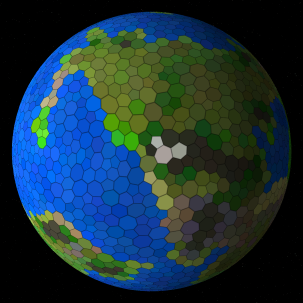
\includegraphics[scale=1]{img/planete.png}
        \caption{Exemple de planète générée procéduralement\protect\footnotemark}
        \label{exemple}
    \end{center}
\end{figure}

\footnotetext{\href{https://experilous.com/1/blog/post/procedural-planet-generation}{https://experilous.com, Procedural Planet Generation Posted on September 30, 2014 by Andy Gainey}}

\newpage 
\section{Analyse de l'existant}

\subsection{Algorithmes de génération de sphère}
\label{algos_gen_sphere}
\subsubsection{Subdivision d'un icosaèdre : icosphére}

Il existe différentes méthodes pour générer une sphère à face polygonale. La toute première est la subdivision à plusieurs reprises d'un  icosaèdre pour obtenir une géode. Un icosaèdre est un polyèdre composé de  12 sommets et 20 triangles équilatéraux (visibile figure  \ref{figure0}). La géode quant à elle est un polyèdre convexe inscrit dans une sphère dont il réalise une approximation. Pour obtenir cette géode, on réalise une subdivision des triangles composant l'icosaèdre en  4 triangles plus petits. On répète cette opération plusieurs fois afin d'obtenir la surface désirée. On peut voir le résultat après 2 subdivisions consécutives sur la figure \ref{figure1}.\\
\\
L'utilisation de cette approche permet d'obtenir une position des points régulière mais aussi une décomposition de la sphère en triangle de même taille sans appliquer d'autres algorithmes supplémentaires (Comme Voronoï ou Delaunay qui sont expliqués plus bas). Il s'agit de la méthode standard. Il est possible d'appliquer cette subdivision sur les uv-spheres et les cubesphéres, mais les polygones ne seront pas identiques, et donc leur taille non plus. Pour plus d'informations, voir la référence \cite{SongHoAhn}. Il est néanmoins possible de partir directement de points et de les relier par la suite. C'est le cas de l'utilisation de la sphère de Fibonacci.\\

\begin{figure}[!h]
    \begin{center}
        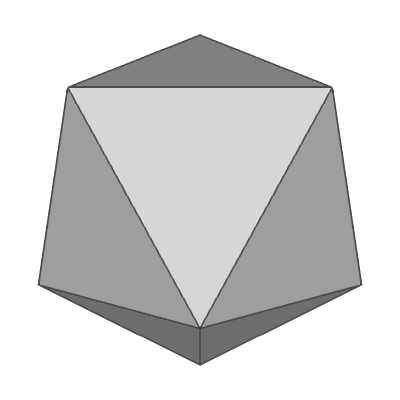
\includegraphics[width=0.2\linewidth]{img/sphere/gl_sphere05.png}
        \caption{Icosaèdre\protect\footnotemark}
        \label{figure0}
    \end{center}
\end{figure}

\footnotetext{\href{http://www.songho.ca/opengl/gl_sphere.html}{http://www.songho.ca/, OpenGL Sphere, 2018 by Song Ho Ahn, Accessed January 2020}}

\begin{figure}[!h]
    \begin{center}
        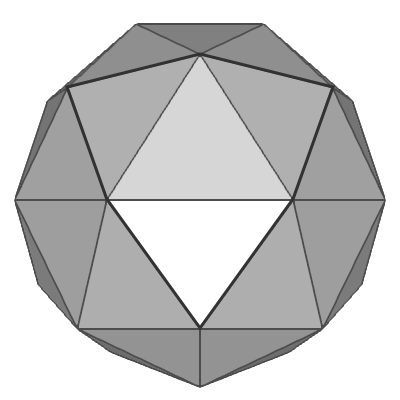
\includegraphics[width=0.2\linewidth]{img/sphere/gl_sphere06-2.png} 
        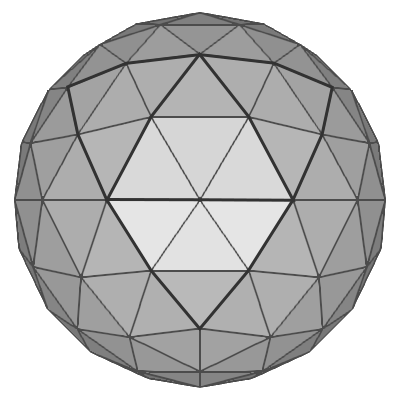
\includegraphics[width=0.2\linewidth]{img/sphere/gl_sphere07-2.png} 
        \caption{Subvidision à 2 reprises d'un icosaèdre.\protect\footnotemark}
        \label{figure1}
    \end{center}
\end{figure}

\footnotetext{\href{http://www.songho.ca/opengl/gl_sphere.html}{http://www.songho.ca/, OpenGL Sphere, 2018 by Song Ho Ahn, Accessed January 2020}}

\subsubsection{Sphère de Fibonacci}

Une sphère de Fibonnacci est la représentation d'une sphère par dispersion de points (voir figure \ref{fibosphere}). Différents algorithmes peuvent être utilisés pour générer cette répartition de points de manière plus ou moins égale. Il y a par exemple celui de la répulsion electrostatique. Il consiste à partir d'une distribution arbitraire des points à appliquer un algorithme de répulsion ponctuelle, dans lequel tous les points se repoussent les uns des autres. On fait alors tourner l'algorithme jusqu'à un certain critère de convergence, autrement dit quand la distribution nous convient. Pour plus d'informations voir \cite{PointDistribution}.
\begin{figure}[!h]
    \begin{center}
        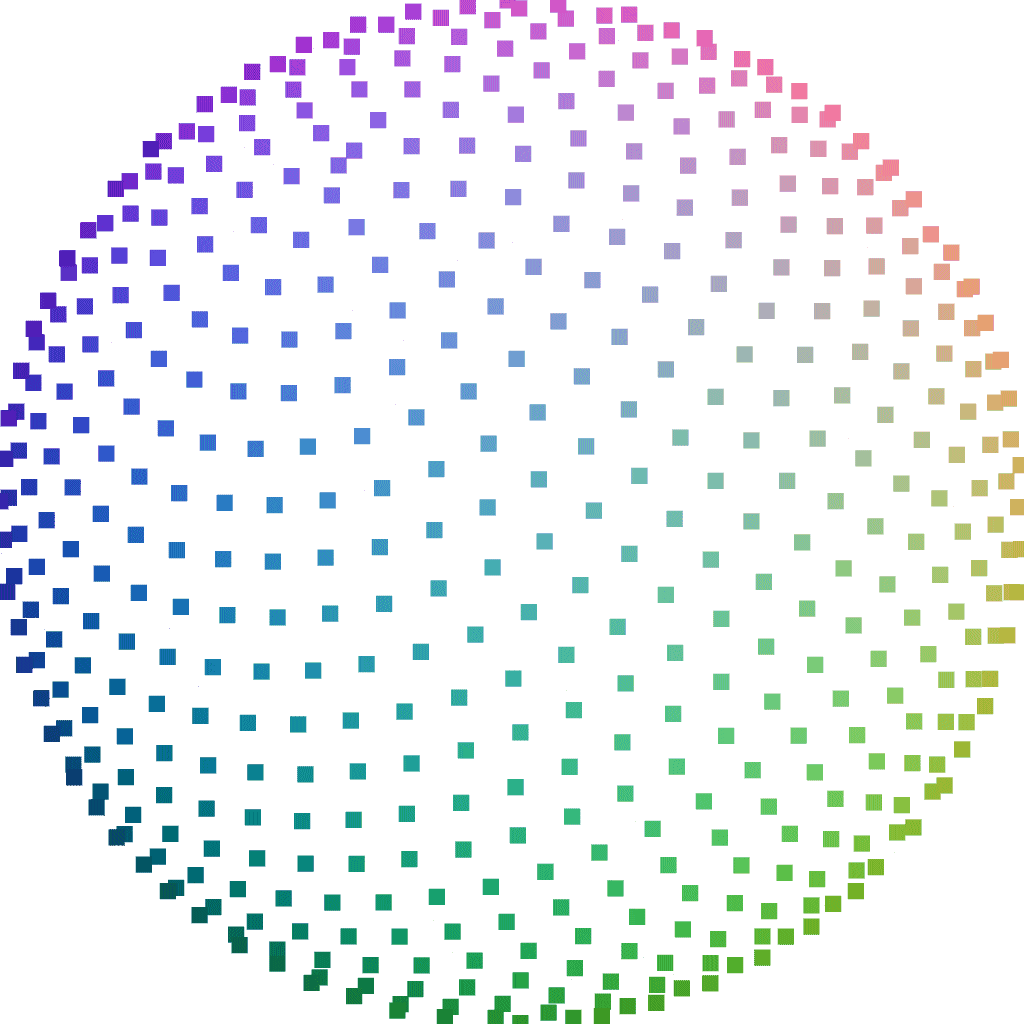
\includegraphics[width=0.5\linewidth]{img/sphere/fibonacci_sphere.png}
    \end{center}
        \caption{Sphère de Fibonacci \protect\footnotemark}
        \label{fibosphere}
\end{figure}

\footnotetext{\href{https://www.redblobgames.com/x/1842-delaunay-voronoi-sphere/}{https://www.redblobgames.com, Delaunay + Voronoi on a sphere
Posted on March 10, 2019 by RedBlobGames, Accessed January 2020}}

Une fois la répartition des points obtenue, il est nécessaire de les relier afin d'obtenir une première version d'une sphère. On peut alors utiliser le tout premier algorithme : La triangulation de Delaunay. Cette triangulation consiste à relier tous les points d'un plan P, tel qu'aucun point de P n'est à l'intérieur du cercle circonscrit d'un des triangles formés. On peut bien sûr étendre cette définition à un espace en 3 dimensions. On parle alors de sphères circonscrites. La sphère finale obtenue est celle de la figure \ref{delaunay}.\\

\begin{figure}[!h]
    \begin{center}
        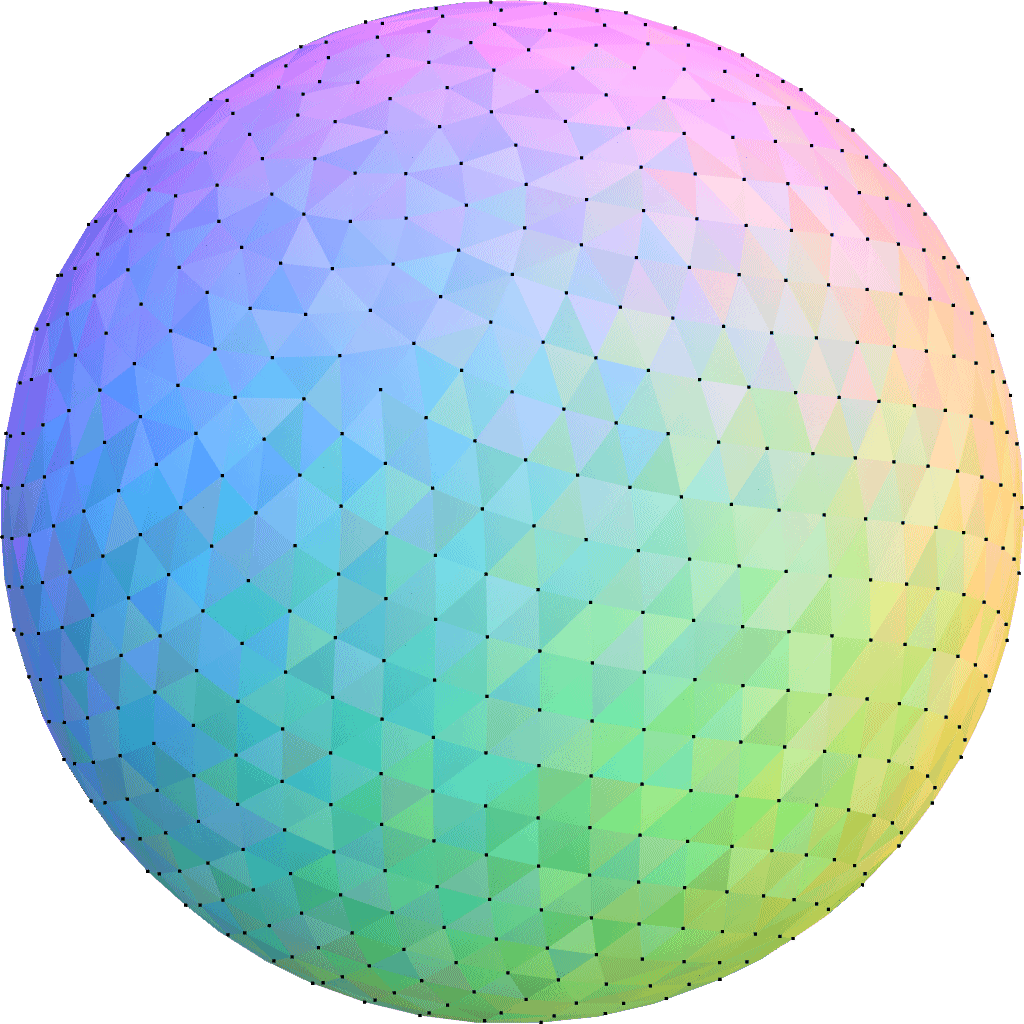
\includegraphics[scale=0.2]{img/sphere/fibonacci-sphere-delaunay.png}
        \caption{Résultat de la triangulation de Delauney pour une sphère\protect\footnotemark}
        \label{delaunay}
    \end{center}
\end{figure}

\footnotetext{\href{https://www.redblobgames.com/x/1842-delaunay-voronoi-sphere/}{https://www.redblobgames.com, Delaunay + Voronoi on a sphere
Posted on March 10, 2019 by RedBlobGames}}

Il est alors facile d'appliquer le diagramme de Voronoï par la suite. Ce diagramme consiste à un pavage (découpage) du plan en cellules. Chaque cellule contient un "germe", représenté par un point, dont la cellule en représente sa zone d'influence. Les sommets du diagramme de Voronoï sont les centres des cercles circonscrits des triangles obtenus par la triangulation de Delaunay. Les arêtes du diagrammes quant à elles sont les médiatrices des arêtes de la triangulation de Delaynay. On peut voir la superposition d'un diagramme de Voronoï et de la triangulation de Delaunay à la figure \ref{superposition}. L'application sur une sphère est présentée à la figure \ref{voronoi}.  Pour plus de détails, il est possible de voir \cite{RedBlobGames}.\\

\begin{figure}[!h]
    \begin{center}
        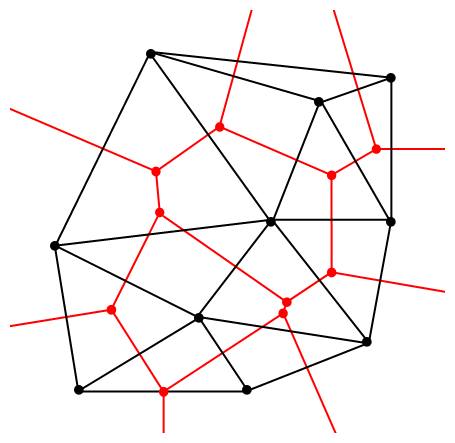
\includegraphics[scale=0.5]{img/Delaunay_Voronoi.png}
        \caption{Superposition d’un diagramme de Voronoï (en rouge) et de la triangulation de Delaunay (en noir).\protect\footnotemark}
        \label{superposition}
    \end{center}
\end{figure}

\footnotetext{\href{https://www.redblobgames.com/x/1842-delaunay-voronoi-sphere/}{https://www.redblobgames.com, Delaunay + Voronoi on a sphere
Posted on March 10, 2019 by RedBlobGames}}

\begin{figure}[!h]
    \begin{center}
        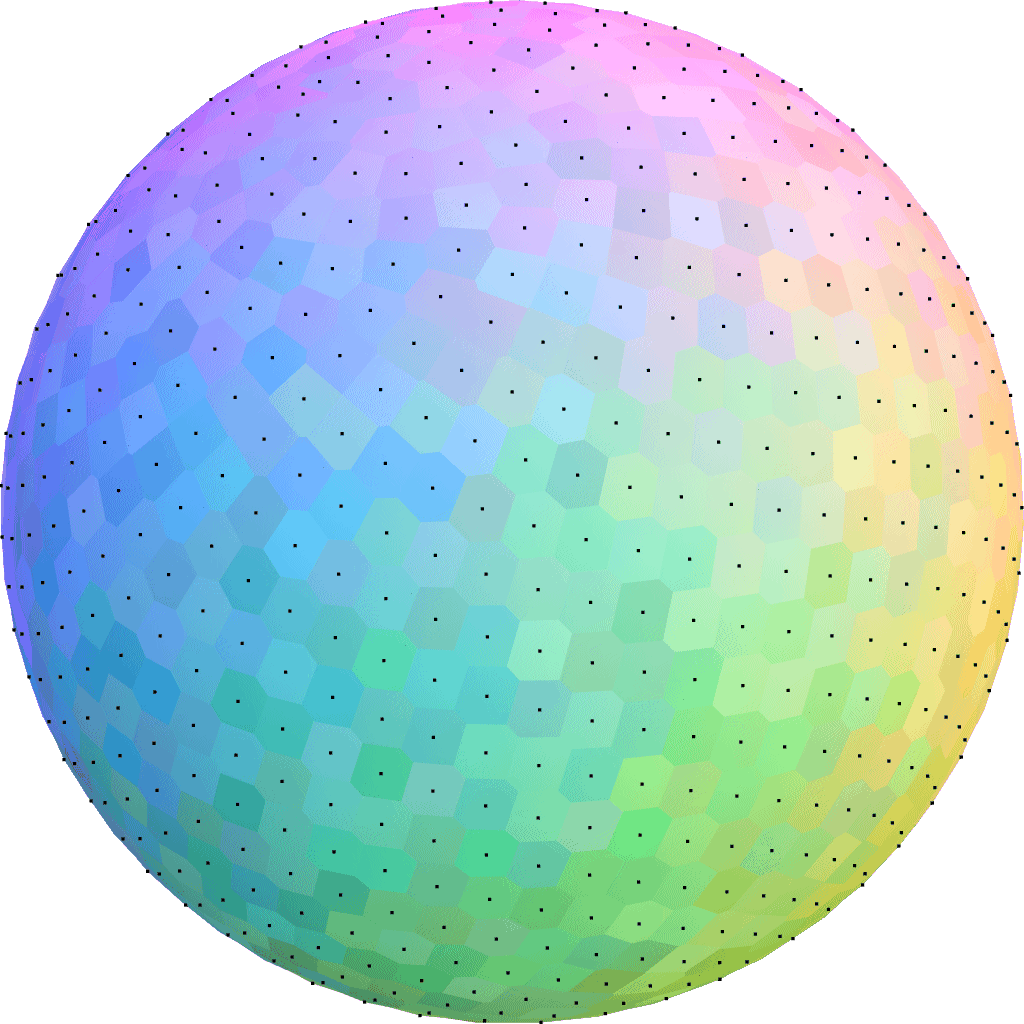
\includegraphics[scale=0.2]{img/sphere/fibonacci-sphere-voronoi.png}
        \caption{Résultat de l'application d'un diagramme de Voronoï sur une sphère.\protect\footnotemark}
        \label{voronoi}
    \end{center}
\end{figure}

\footnotetext{\href{https://www.redblobgames.com/x/1842-delaunay-voronoi-sphere/}{https://www.redblobgames.com, Delaunay + Voronoi on a sphere
Posted on March 10, 2019 by RedBlobGames}}
\newpage
\newpage
\subsection{Algorithmes de générations procédurales aléatoires}
\label{noise_algos}
    Il existe des algorithmes souvent utilisés dans l'industrie du jeu vidéo et de la modélisation 3D permettant de générer procéduralement à partir de textures avec une part d'aléatoire, des environnements plus ou moins réalistes comme des terrains, des nuanceurs ("shader" en anglais), etc. Un exemple est présent sur la figure \ref{figure5}.\\
    
    \begin{figure}[!h]
        \begin{center} 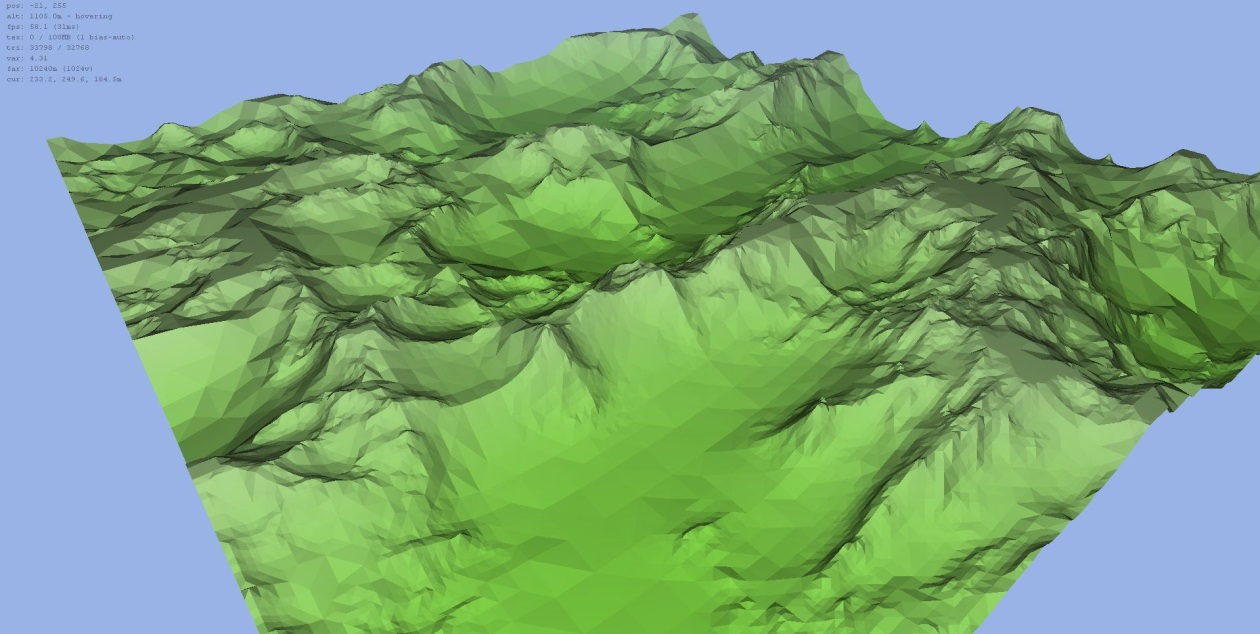
\includegraphics[width=0.8\linewidth]{img/landscape.jpg} \end{center}
        \caption{\label{figure5}Image de terrain généré procéduralement\protect\footnotemark .}
    \end{figure}
            
    \footnotetext{\href{https://sainarayan.me/2015/05/13/procedural-terrain-generation-using-perlin-noise-and-machine-learning/}{https://sainarayan.me, Procedural Terrain Generation
Posted on May 13, 2015 by Cyber Shaman}}
        
    Ces algorithmes se basent sur le modèle du "bruit" mathématique utilisé dans la théorie des signaux, mais avec des paramètres qui permettent de varier les effets. C'est ce qu'on appelle le "chaos", de l'aléatoire contrôlé.\\
    Un exemple très simple serait le bruit dit "blanc"(figure \ref{whitenoise}), ne faisant pas partie de ces bruits chaotiques et est purement aléatoire. Il est peu intéressant pour générer des environnements réalistes, et c'est pour cela que l'on écartera tous les bruits que l'on ne peut pas contrôler.\\
    
        \begin{figure}[!h]
        \begin{center} 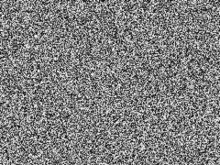
\includegraphics[width=0.4\linewidth]{img/noise/whitenoise.png} \end{center}
        \caption{\label{whitenoise}Image de bruit blanc\protect\footnotemark .}
        \end{figure}
            
        \footnotetext{\href{https://upload.wikimedia.org/wikipedia/commons/thumb/f/f6/White-noise-mv255-240x180.png/220px-White-noise-mv255-240x180.png}{Image from wikipedia}}
        
    Il reste trois types de bruits qui peuvent être intéressant pour ce projet : les bruits de valeurs, les gradients de bruits (Perlin Noise, Simplex Noise), et les bruits organiques (Voronoï, Worley) que l'on peut voir figure  \ref{noises}. Cependant vu la diversité des différents bruits qui existe, le plus intéressant est le bruit de Perlin. Il est le plus utilisé pour réaliser des reliefs de terrain. Il a l'avantage d'être très flexible sur les paramètres donnés, tout en produisant des textures réalistes. Il existe aussi une amélioration moins coûteuse en ressources, Simplex Noise, et qui fait moins d'anormalité sur le rendu 3D (artéfact). Pour plus d'informations, lire \cite{BookShader}.\\

    \begin{figure}[!h]
    \begin{center}
    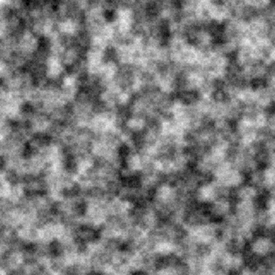
\includegraphics[width=0.4\linewidth]{img/noise/value.png}
    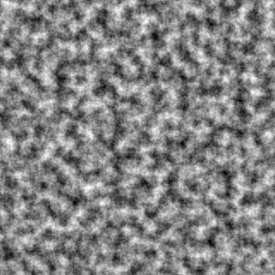
\includegraphics[width=0.4\linewidth]{img/noise/perlin.png}
    \end{center}
    \begin{center}
    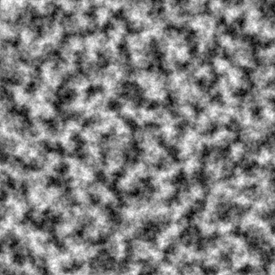
\includegraphics[width=0.4\linewidth]{img/noise/simplex.png}
     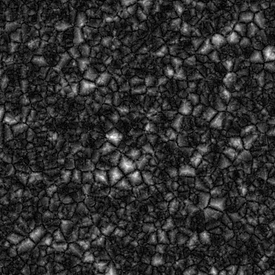
\includegraphics[width=0.4\linewidth]{img/noise/voronoi.png}
     \end{center}
     \begin{center}
    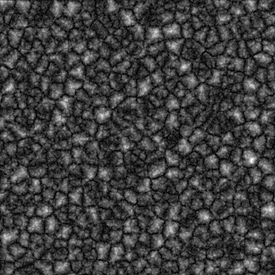
\includegraphics[width=0.4\linewidth]{img/noise/worley.png}
    \end{center}
        \caption{\label{noises}Différents types de bruit\protect\footnotemark.\\
        A partir d'en haut à gauche jusqu'en bas à droite : valeur, Perlin, Simplex, Voronoï, Worley.}
    \end{figure}

    \footnotetext{\href{https://github.com/Scrawk/Procedural-Noise}{Image d'une bibliothèque Github par l'utilisateur Scrawk, Accessed January 2020}}

\newpage
\subsection{Rendu graphique 3D} \label{raster/ray}

Il existe deux méthodes principales pour le rendu d'une scène 3D : la rastérisation et le ray tracing.

            La rastérisation est un procédé qui consiste à convertir une image vectorielle en une image matricielle destinée à être affichée sur un écran. On englobe dans la rastérisation tous les procédés permettant d'améliorer l'aspect final du rendu en 3 dimensions.
            Les objets à l'écran sont créés à partir de triangles ou de polygones qui définissent le modèle 3D de l'objet.
            \begin{itemize}
                \item \textbf{Avantages :}
                \begin{itemize}
                    \item Faible coût en mémoire,
                    \item Plus de choix dans la représentation des faces et du modèle (triangles, quadriques, polygones, torres ...),
                    \item La performance dépend directement du nombre de faces.
                \end{itemize}
                \item  \textbf{Inconvénients :}
                \begin{itemize}
                    \item Rendu simplifié non réaliste,
                    \item Ne prend pas en compte les reflets, la transparence, l'effet miroir.
                \end{itemize}
            \end{itemize}
        
Une autre méthode existante est le ray tracing qui remédie aux inconvénients de la rastérisation. Cette technique reproduit les phénomènes physiques que sont la réflexion et la réfraction. Cela permet un rendu plus réaliste en tenant compte de la lumière, des reflets ou encore de la transparence. Cependant, il s'agit d'avantages qui ne correspondent pas aux besoins clients. Il a donc été décidé de ne pas se pencher sur cette technique de rendu et d'utiliser la rastérisation.
        
\subsection{Outils existants et prototypes}

\subsubsection{Blender}

Afin de pouvoir générer et afficher la planète, une des solutions qui peut-être abordée est l'utilisation d'outils de modélisation en 3 dimensions. Ils disposent déjà de moteurs de rendu performant, dont certains utilisent un système de scripting et de plugin afin de générer des formes, les modifier, et les texturer, pour ensuite les utiliser plus tard dans d'autres logiciels, selon des formats standardisés.

L'un de ces outils existant est l'outil Blender. Il est tout d'abord un logiciel open source, dont le moteur interne est en C/C++ permettant de bonnes performances. Il dispose aussi d'une API en Python permettant un prototypage très rapide.

Un script python a été écrit permettant de :
\begin{enumerate}
            \item {créer une icosphère d'environ 10 000 polygones}
            \item {appliquer une transformation sur ses sommets selon une texture de Voronoï.}
            \item {afficher les paramètres et le temps de génération.}
\end{enumerate}

Le script est disponible dans la hiérarchie du projet \textit{docs/requirements/test\_blender} ainsi que les résultats. Le premier résultat obtenu en exportant l'image depuis l'éditeur est visible sur la figure \ref{blendericos}.\\

\begin{figure}[!h]
\begin{center} 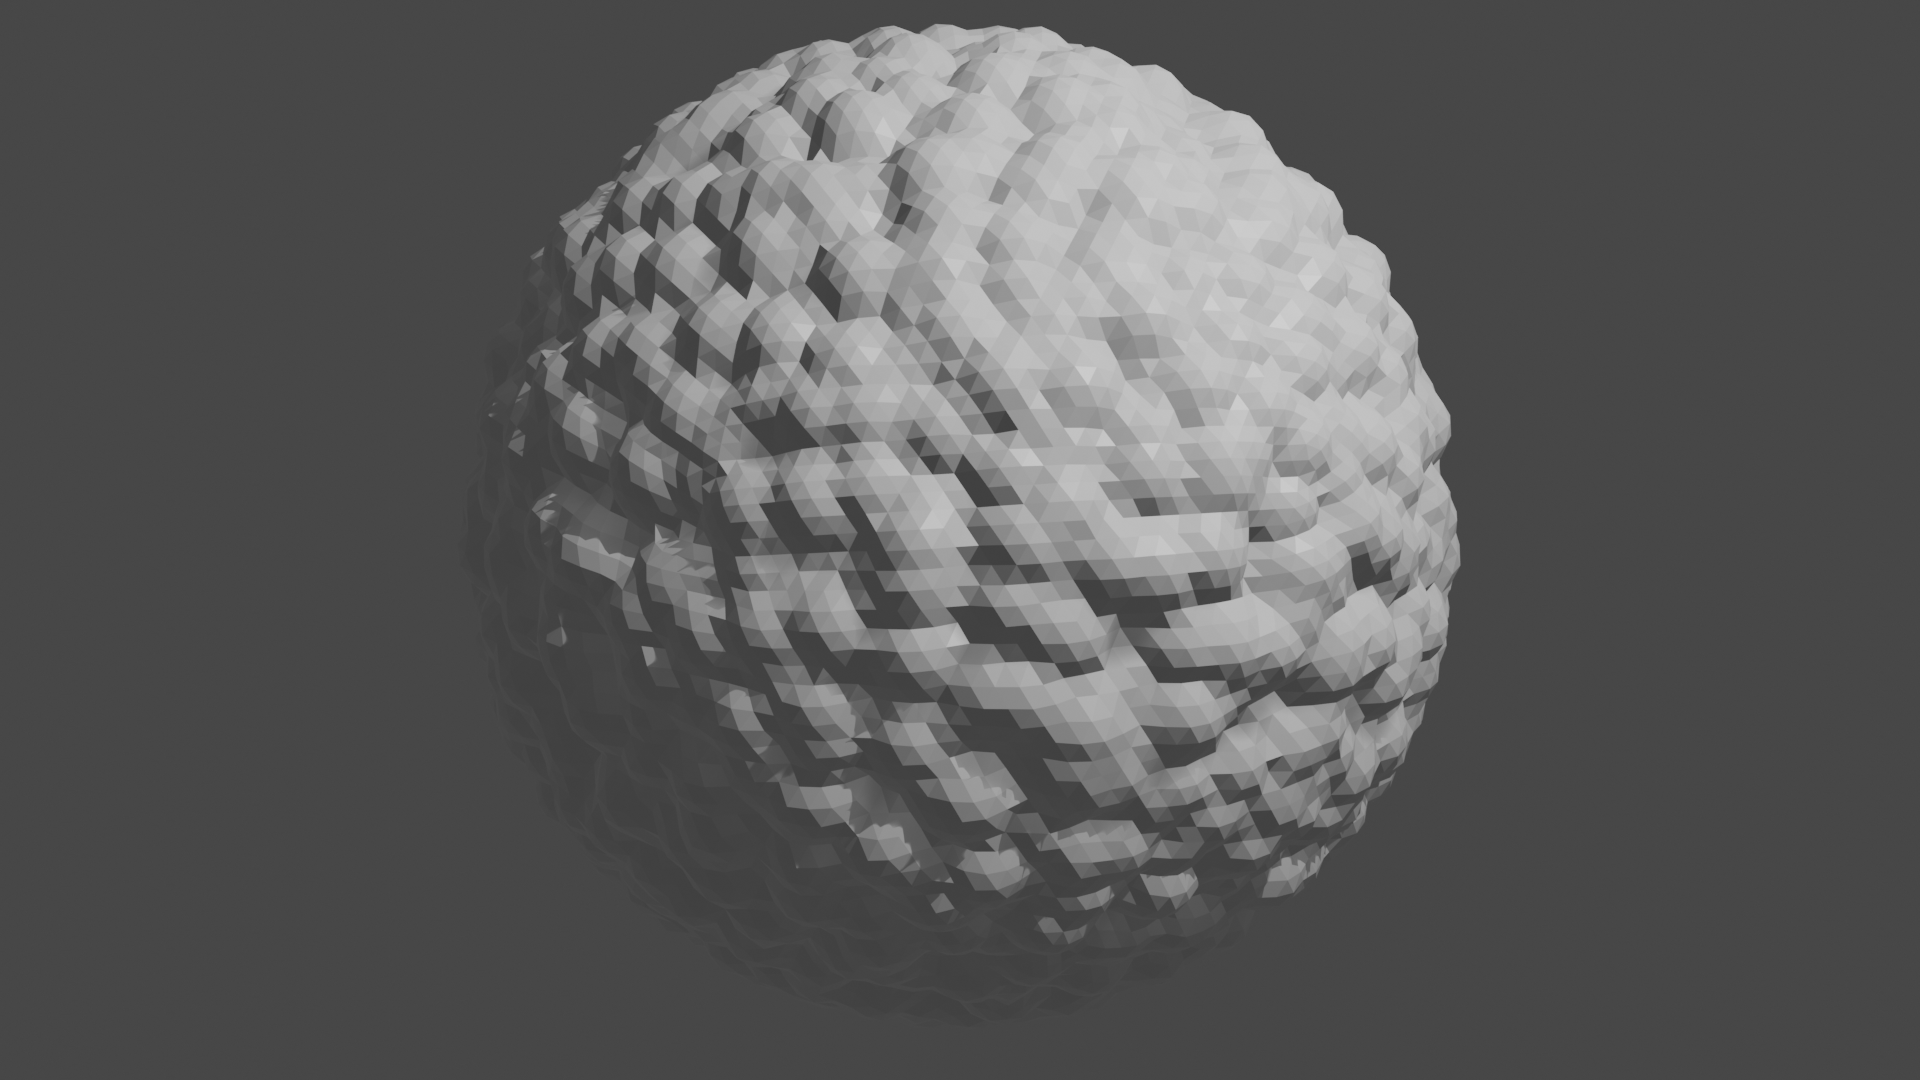
\includegraphics[width=0.6\linewidth]{img/blender/blender_1.png} \end{center}
\caption{\label{blendericos}Icosphère générée par Blender. Texture de bruit Voronoï, 6 subdivisions, \textasciitilde0.02 s, 20480 polygones}
\end{figure}

Attention à la version de Blender. Le moteur de rendu utilisé est Evee version 2.8 permettant une visualisation sans dégradation lors du déplacement de point de vue (rotation, zoom) avec les rendus finaux. Pour des soucis de performance, il faut aussi faire attention à la machine utilisée, notamment la carte graphique.\\

Les paramètres ont été changés depuis l'éditeur Blender afin d'arriver aux résultats figure \ref{blendericosmodif} et \ref{blendericosmodifedit}.\\

\begin{figure}[!h]
\begin{center} 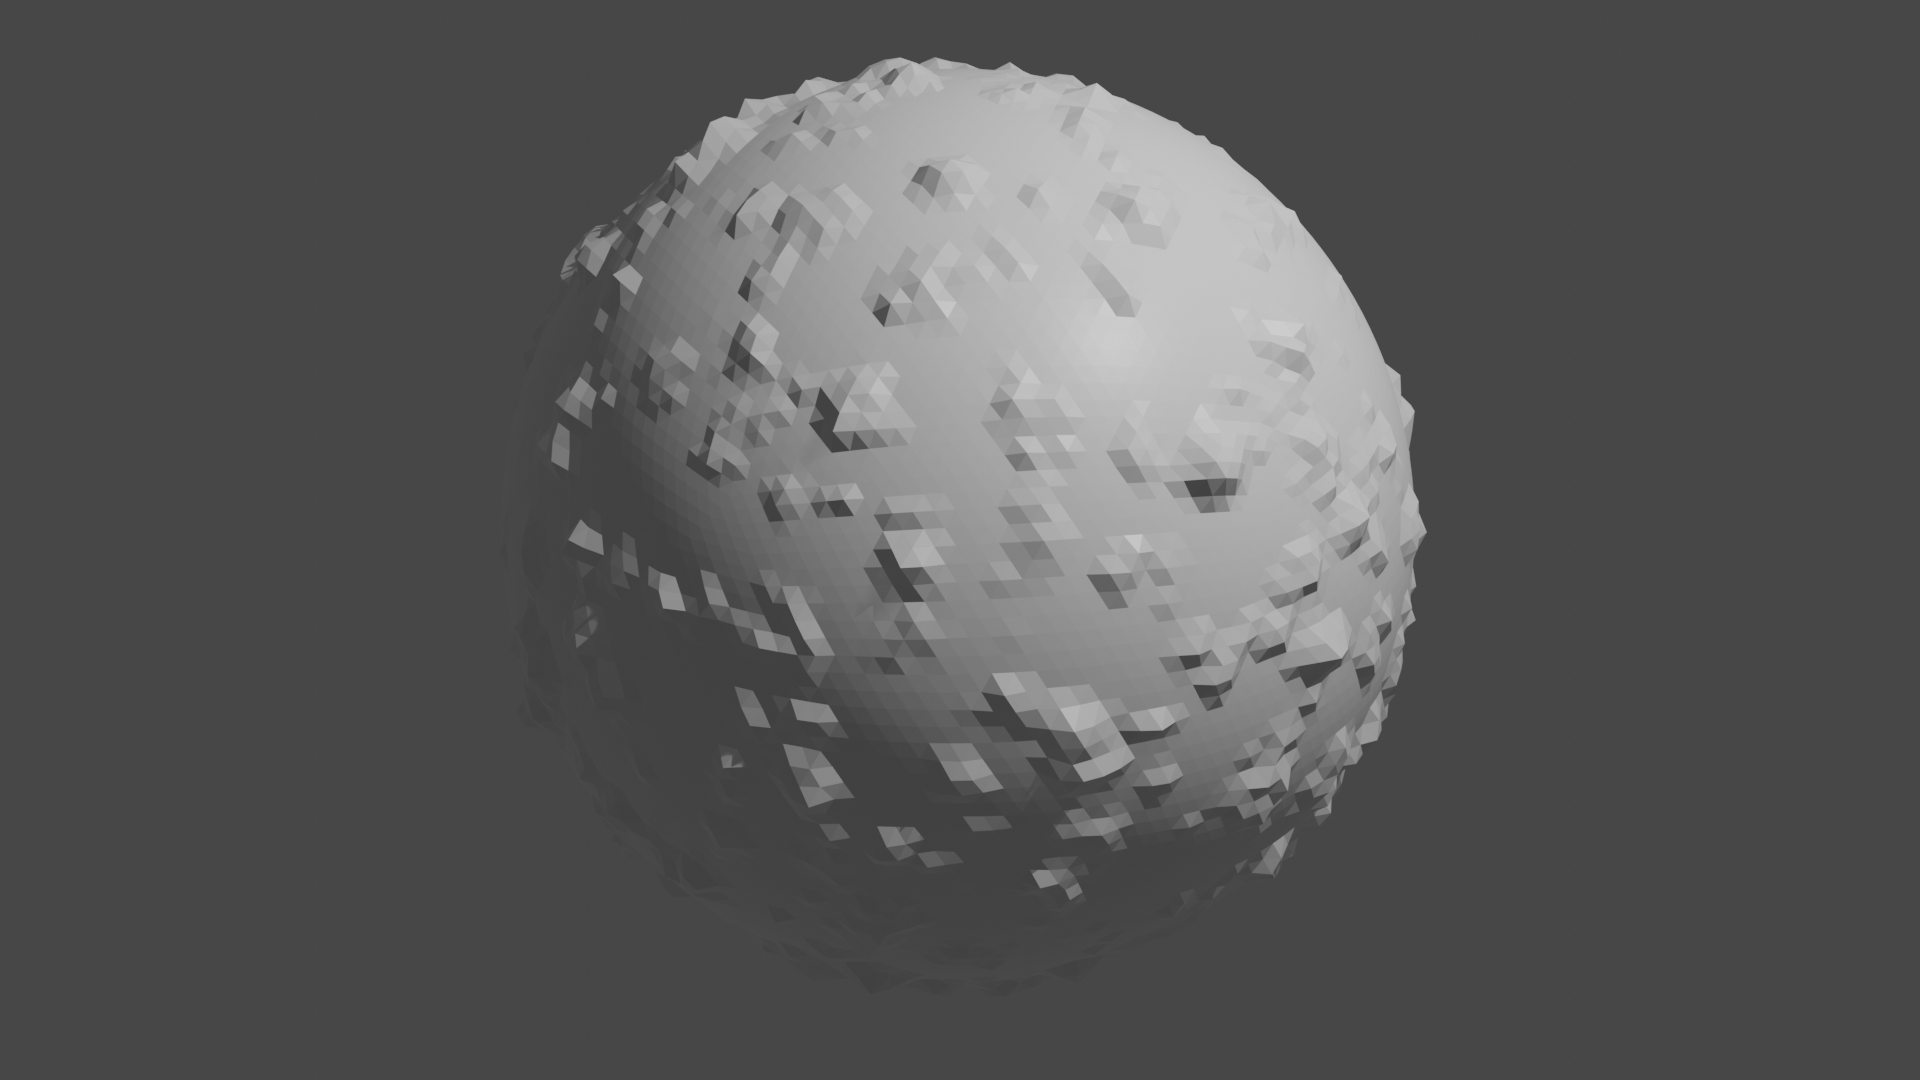
\includegraphics[width=0.6\linewidth]{img/blender/blender_2.png} \end{center}
\caption{\label{blendericosmodif}Modification de la texture de bruit Voronoï sans couleur}
\end{figure}

\begin{figure}[!h]
\begin{center}
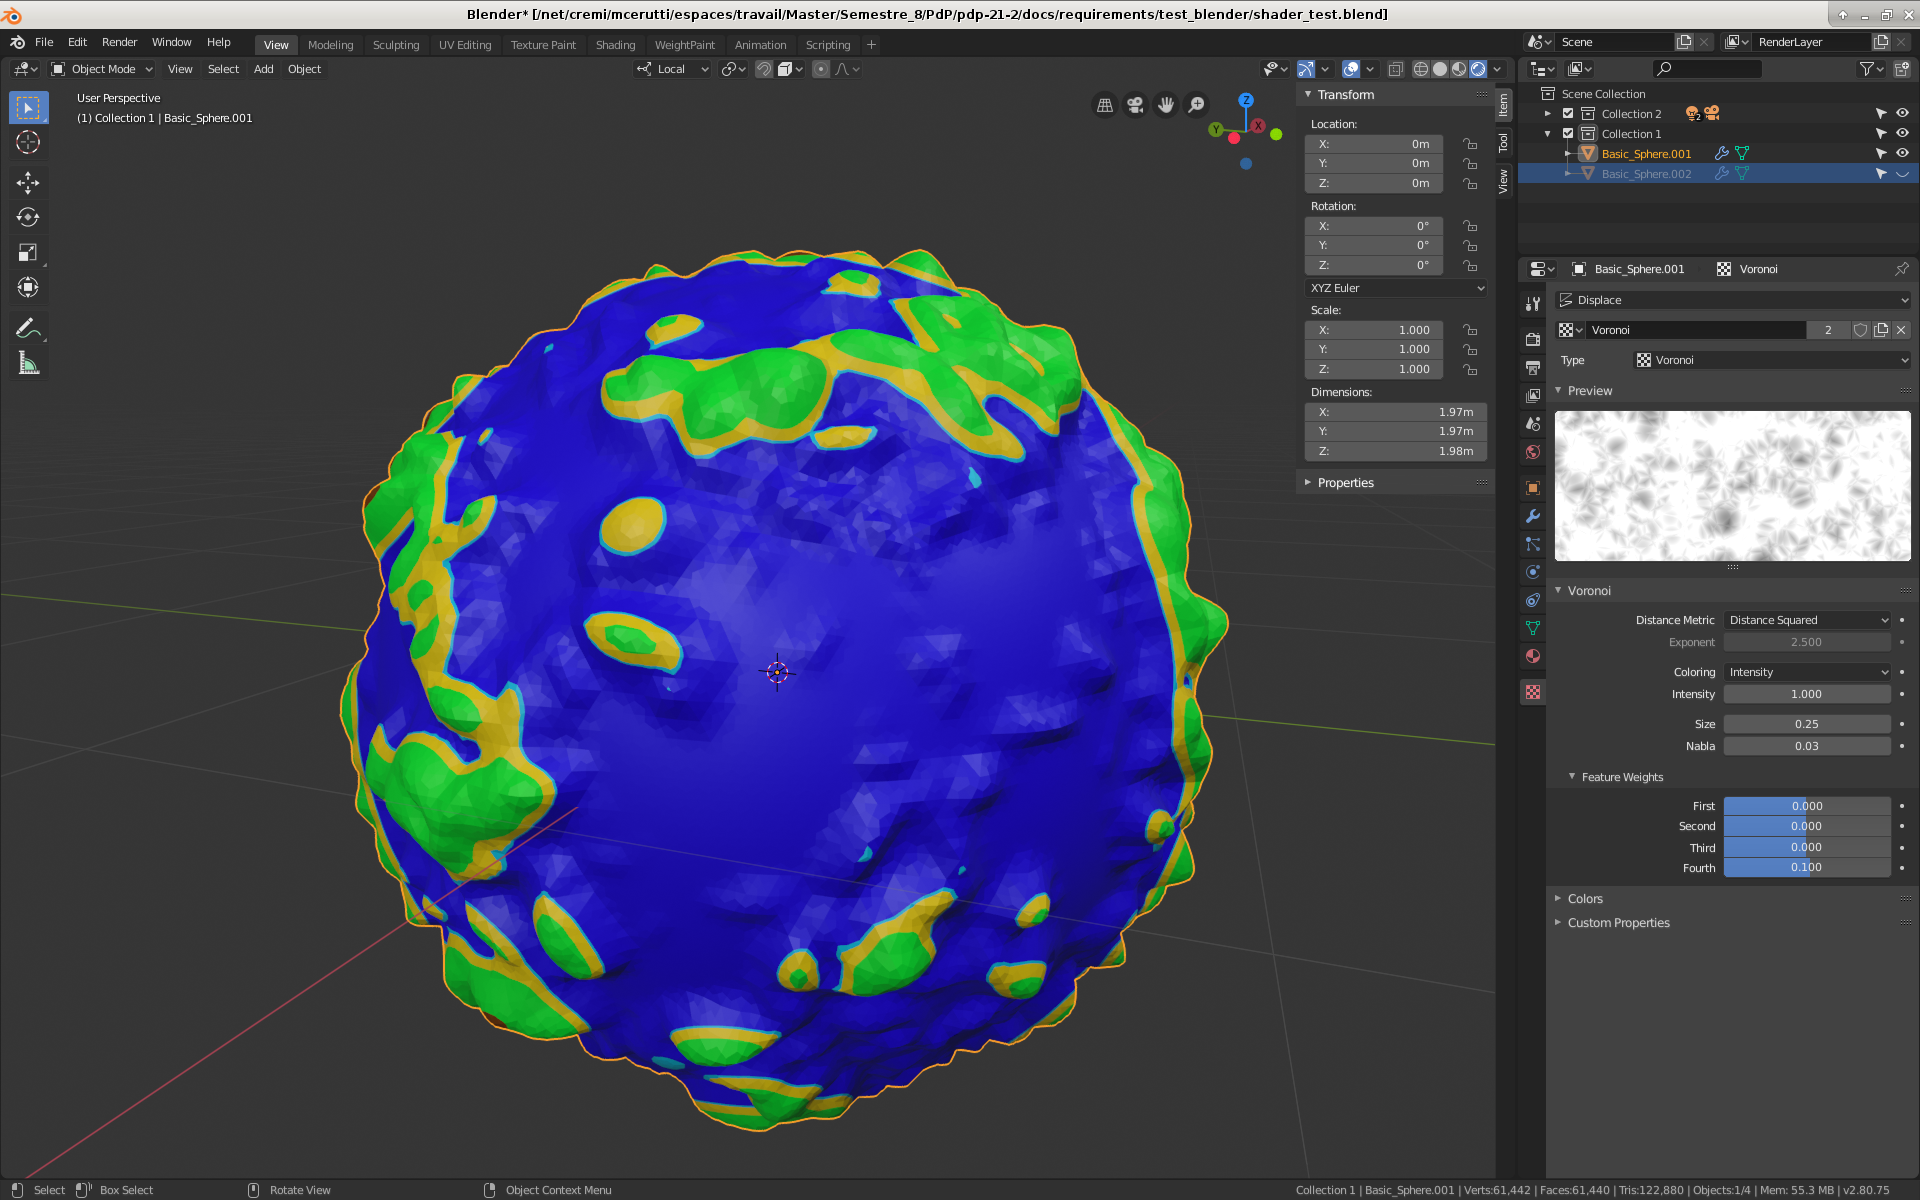
\includegraphics[width=0.6\linewidth]{img/blender/blender_editeur_bruit.png}
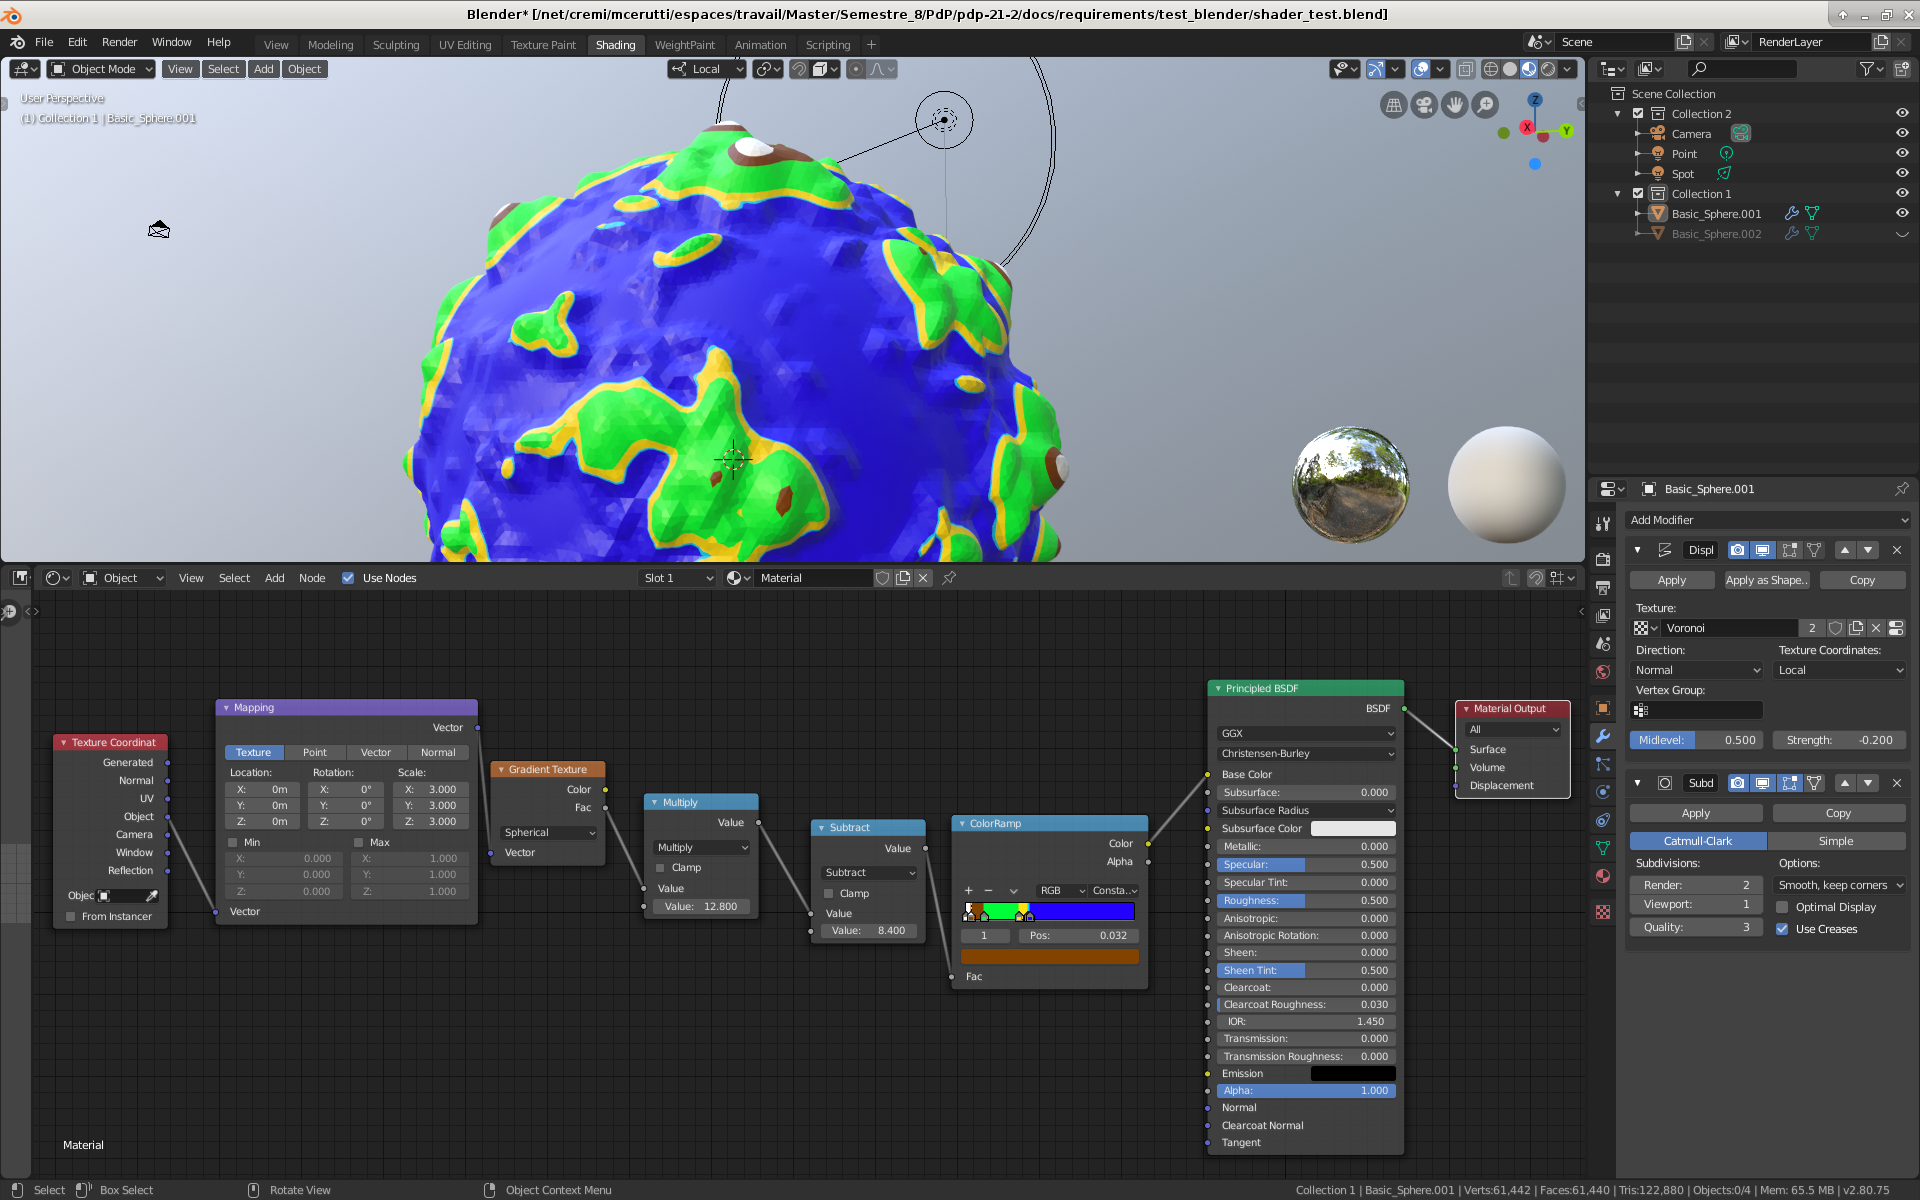
\includegraphics[width=0.6\linewidth]{img/blender/blender_shaderEditor.png}
\end{center}
\caption{\label{blendericosmodifedit}Essais de modifications par l'éditeur Blender : paramètres de texture, bruit de déplacement des sommets, rajout de nuances (shader)}
\end{figure}

\newpage
\paragraph{Avantages}

\begin{enumerate}
            \item {Rendu de base avec OpenGL, Moteur interne en C/C++ :}
            Permet d'espérer de très bonnes performances au niveau des algorithmes de base. Crucial dans le cas de rendu de l'ordre de 60 images par secondes (FPS) avec une bonne machine.
            
            \item {Open source et sous GNU General Public License (ou "logiciel libre") :}
            Cela permettrait de modifier le moteur de rendu, et les algorithmes de visualisation selon les besoins.
            
            \item {Multi-plateforme :}
            Permet le portage Linux (correspondant à notre besoin), et aussi sur d'autres plateformes nativement.
            
            \item {API très simple en Python afin d'accéder et de modifier la forme :}
            Permet de faire des tests très rapides, et de laisser le client manipuler les algorithmes de modification plus facilement qu'on aurait implémenté en sur-couche du moteur interne.
            
            \item {Fonctionnalités supplémentaires (sauvegarde, modification, amélioration de rendu, création de nuauceurs en noeuds...) :}
            Permettrait de se focaliser davantage sur les fonctionnalités concernant la génération de la planète, en ayant déjà les possibilités d'extensions de notre projet.
            
\end{enumerate}

\paragraph{Inconvénients}

    \begin{enumerate}
                
                \item {Ne convient pas à l'exercice du PDP :}
                étant informaticiens et non des graphistes, il n'y a aucun intérêt pédagogique à utiliser un outil aussi complet. Son utilisation nécessiterait aucunement une équipe de 5 personnes, et encore moins au sein d'une formation informatique.
                
                \item {Interface de Blender trop riche pour le client :}
                contraire à la demande du client demandant une visualisation simple. Nécessite une connaissance au moins de surface de l'outil. Risque de refus à envisager avant de commencer à l'utiliser.
                
                \item {La version de Blender influe sur l'API (la version 2.8 n'est pas encore formellement documentée), et sur les performances de rendu (moteur Evee) :}
                risques d'instabilité et de bug sur l'API fournie, ainsi qu'un développement plus chaotique du fait d'un manque de documentation.
                
                \item {Pas de sécurité sur des paramètres trop grands (cesse de fonctionner, pas d'erreurs de ressources si demande trop grande) :}
                lié au fait d'utiliser une API en "boîte noire", nécessite un apprentissage des fonctions du moteur interne et une bonne documentation. Cela aussi influe sur la flexibilité du code et les limites d'extensions avec le logiciel de base.
                
                \item {Rendu et génération dépendant de la machine choisi :}
                il est nécessaire d'avoir une configuration suffisamment puissante pour pouvoir utiliser cet outil (se référer à la configuration du client \ref{Compatibilité}).
                
    \end{enumerate}
    
\subsubsection{OpenGL}
\label{choixoutil}
OpenGL (Open Graphics Library) est considérée comme une API (Application programming interface) qui offre la capacité d'afficher des objets en 2D et en 3D. Elle est principalement utilisée pour interagir facilement avec les cartes graphiques (GPU). Elle est utilisée en C/C++. Néanmoins, c'est avant tout une spécification, qui décrit ce que sont les entrées et sorties de chaque fonction et comment elles doivent s'exécuter. Cette spécification est implémentée par les constructeurs de carte graphique (dans les pilotes). OpenGL est disponible sous plusieurs versions.
La version 3.3 quant à elle, est une base de la programmation moderne d'OpenGL (et donc actuellement la plus utilisée) et permet une grande flexibilité et efficacité. Qui plus est, les versions supérieures à celle-ci implémentent des fonctionnalités supplémentaires sans changer les précédentes. Il y a donc un faible problème de compatibilité. Il est tout à fait possible d'afficher une sphère de plus de 10 000 polygones, comme le prouve la figure \ref{sphereOpenGL}.

\begin{figure}[!h]
\begin{center}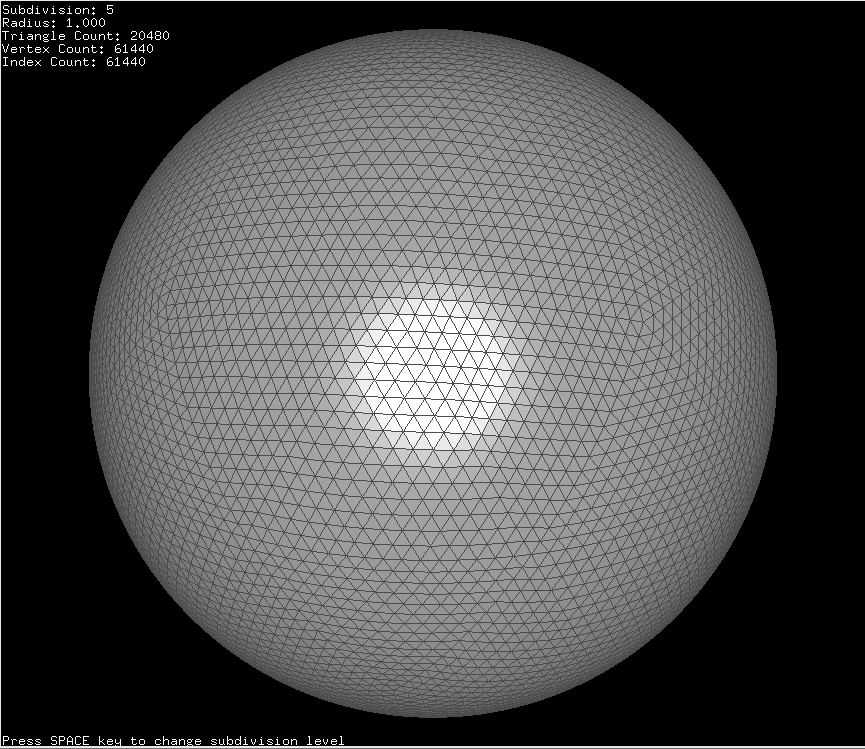
\includegraphics[width=0.6\linewidth]{img/icosphere.png} \end{center}
\caption{Affichage d'une sphère en OpenGL avec plus de 10000 polygones}
\label{sphereOpenGL}
\end{figure}

\paragraph{Avantages}
    \begin{enumerate}
                \item {Performant :}
                Ces bibliothèques sont implémentées en C/C++ et sont utilisées par de nombreuses compagnies, studios et équipes de développement afin de faire des applications graphiques performantes (60 images par secondes et définition 4K maintenant). On peut donc espérer avoir de bonnes performances concernant le logiciel.
                
                \item {Accessible :}
                Les principales bibliothèques dérivées d'OpenGL ont une bonne documentation et de nombreux tutoriels. Cela permet d'avoir plus de temps pour l'implémentation sachant que l'apprentissage sera plus aisé.
                
    \end{enumerate}

\paragraph{Inconvénient}
    \begin{enumerate}
                \item {Temps de développement :}
                Du fait que OpenGL est en C/C++, la réfléxion pour la gestion mémoire et l'architecture demandera du temps. Il sera donc nécessaire d'avoir ces faits en tête lors du développement.
                
                \item {Complexité de prise en main :} 
                OpenGL et ses bibliothèques offrent une très grande flexibilité mais la compréhension et la prise en main de celles-ci est très complexe, comme il y en a beaucoup. Même avec les bons tutoriels et une bonne documentation, il faudra prendre en compte l'apprentissage dans le temps passé au développement.
                
    \end{enumerate}
    

\subsubsection{Gestion de fenêtre et interaction utilisateur}
    OpenGL ne permet pas directement de gérer des fenêtres et des évènements d'entrée (clavier/souris). En revanche, il existe principalement deux bibliothèques open source qui étendent OpenGL et permettent cela : freeglut\cite{freeglut} (écrit en C et sous licence X-Consortium) et GLFW\cite{GLFW} (écrit en C et sous licence zlib/libpng).\\
    
    Ces bibliothèques mettent des fonctions à disposition dont la création de fenêtre en indiquant ses dimensions. Il faut ensuite utiliser une boucle de rendu pour garder la fenêtre ouverte, continuer de dessiner les images et gérer les entrées utilisateur.\\
    
    Il n'y a pas vraiment de différence de fonctionnalité entre ces deux bibliothèques, si ce n'est que freeglut est basé et étend la bibliothèque GLUT qui était très utilisé par le passé mais sous droit d'auteur privé et dépassé.

      
 \subsubsection{Bibliothèques de bruit}
    
    Il existe des bibliothèques permettant justement d'implémenter les différents algorithmes vue dans la partie \ref{noise_algos} dans différents languages.
    Celles qui nous ont le plus attiré notre attention sont Libnoise \cite{LibNoise} et FastNoise \cite{FastNoise} en accord avec les choix précédents.\\

    Libnoise est une bibliothèque sous licence GNU LESSER GENERAL PUBLIC LICENSE Version 2.1 en C++, portable, et qui a un de nombreuses ressources pour la prendre en main. C'est aussi la bibliothèque la plus utilisé à ce jour. Elle permet aussi avec du code utilitaire associé d'exporter les bruits sous forme de texture d'image, et même d'appliquer des traitement plus complexes en combinant les bruits, rajoutant des gradients de couleurs. Un exemple complet est montré figure \href{libnoiseExample}.\\
    
    \begin{figure}[!h]
        \begin{center} 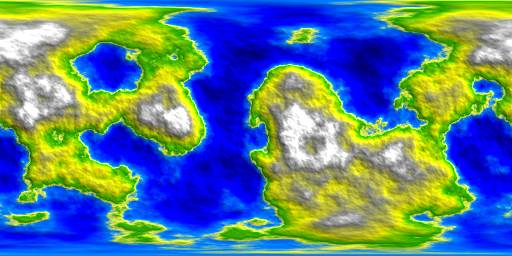
\includegraphics[width=0.8\linewidth]{img/noise/libnoise_sphericalheightmap.jpg} \end{center}
        \caption{\label{libnoiseExample}Exemple d'une texture sphérique créé avec libnoise\protect\footnotemark .}
        \end{figure}
    
    \footnotetext{\href{http://libnoise.sourceforge.net/tutorials/tutorial8.html}{Image du tutoriel numéro 8, Accessed Marsh 2020}}
    
    La bibliothèque FastNoise quant à elle est sous MIT License, et est disponible dans différents langages, C++, C\# et aussi sous instructions SIMD. Elle est beaucoup plus récente que la précédente est a notamment de bonnes performances et est plus rapide que libnoise \protect\footnotemark.\\
    
    \footnotetext{Selon les chiffres donnée par la page : \href{https://jordanpeck.me/2016/05/fastnoise/}{https://jordanpeck.me/2016/05/fastnoise/}}
    
 \subsubsection{Moteurs de jeux}

    Il est possible de s'intéresser aux moteurs de jeux. Le seul moteur de jeu qui aurait pu être intéressant est Godot, car il est open source et est sous licence MIT qui a des avantages au niveau de la distribution et de son utilisation comparé aux concurrents les plus utilisé Unity et Unreal Engine. Mais cette solution a été vite écartée pour trois grandes raisons : 
    \begin{enumerate}
        \item  La première est que les moteurs de jeux, bien qu'ils aient un moteur de rendu 3D intégré sont beaucoup trop fournis en fonctionnalités. La plupart des fonctionnalités ne sont pas intéressantes pour ce projet. 
        
        \item La deuxième est que cela ne convient pas à l'exercice du PDP, en soit faire une sur-couche et faire quelques modifications aurait suffi, mais ce n'est pas le but pédagogique de PDP.
        
        \item  La dernière est que bien que le moteur de rendu permet d'avoir déjà des optimisations, il risque d'y avoir encore plus de code qui peut ralentir le rendu. Pire, cela rajoute des dépendances et l'installation d'un moteur de jeu par le client, ce qui est contraire à une interface simple.
    \end{enumerate}

 \subsubsection{Cours Université}
    
    On s'est intéressé en parallèle du développement au cours de "Mondes 3D" du professeur Pierre BÉNARD en Master 1 Informatique, filière IIS de l'université de Bordeaux. Notamment cela a notamment permis d'avoir une base de code pour l'outil OpenGl avec la théorie qui va avec. Avec sa permission, nous avons pu récupérer les ressources pour notre projet \cite{TD_3D}.

\newpage 
\section{Besoins}

Les besoins fonctionnels et non fonctionnels seront énoncés, ainsi que la manière d'y répondre.

\subsection{Besoins fonctionnels}

\subsubsection{Génération d'une planète}

\subsubsubsection{Géométrie de la planète}
\label{geo_planet}
La planète est caractérisée par une sphère. Il doit donc être nécessaire de pouvoir créer une sphère. L’analyse de l’existant à montrer qu’il existait plusieurs techniques avec deux approches de départ différentes : avec des points, ou directement avec des formes.  La solution la plus adéquat est l’utilisation de l’icosaèdre avec sa subdivision. C’est une méthode tout à fait standard et efficace qui ne nécessitera pas l’implémentation d’algorithmes supplémentaires pour un rendu minimal correct à l’inverse de la sphère de Fibonnaci. Qui plus est, l’implémentation et l’utilisation d’algorithmes supplémentaires pour améliorer le rendu est tout à fait envisageable avec l’utilisation de l’icosaèdre. C'est pour cela que nous avons choisi cette solutions au vu de l'ensemble des avantages qu'elle présente.

\subsubsubsection{ Représentation des informations }
La géométrie définit précédemment, en soit une sphère quasi-parfaite, sert forme de base à notre planète. Ce n’est que après que l'on peut la modifier à notre guise. Ce qui amène du coup à la définition même des informations que l’on va créer et représenter. Dans notre cas, il a été choisi de ne pas créer d'informations supplémentaires et se de contenter d'utiliser la notion de position et de couleurs offertes par les points. La planète ne se voulant pas être une simulation réaliste, il n'a pas été nécessaire de mettre en place des pôles, un équateur, des biômes et une logique scientifique vis à vis de la position des reliefs (plaques tectoniques). 

\subsubsubsection{Paramètres modifiables}
\label{besoin_paramètres}
Les informations générées doivent en partie être contrôlé par l'utilisateur. Si il veut, il doit pouvoir fixer certains paramètres de la génération, ou au contraire, les laissé aléatoire avec un moyen de contrôle sur eux. Ces paramètres pourrait être changer à chaque exécution du logiciel sans recompilation, mais pas dynamiquement une fois que la planète est crée. Nous avons choisi pour cela de faire un système de fichier de configuration avec un parseur en XML grâce à la bibliothèque pugyXML, afin de de pouvoir lire et changer les paramètres à l'exécution.

\subsubsubsection{Gestion de l'aléatoire}
\label{besoin_aleatory}
Comme dit précédemment, certains paramètres pourraient être géré aléatoirement, mais il doit être possible de recréer la même planète, au au moins une dont les caractéristiques se rapprochent.
Il faut donc communiquer aussi ces informations à l'utilisateur pour qu'ils puissent les modifier s'il le souhaite. 
Pour des paramètres simplement aléatoire de type "bruit blanc"(random), la bibliothèque standard suffit, pareil pour des lois de distribution classique comme la distribution gaussienne, où on peut afficher cependant l'information de la graine aléatoire (seed). Pour de l'aléatoire plus réaliste, la bibliothèque Libnoise choisi permet justement de générer des bruits avec les propriétés qui nous intéressent dit précédemment.

\subsubsection{Visualisation d'une planète}
% TODO

\subsubsubsection{Affichage de la planète}
Une seule planète doit être affichée à la fois.  Afin d’y parvenir, il fallait donc créer une fenêtre (éventuellement extensible) qui se lancera lors de l’appel à l’exécutable. Étant donné la visée ludique de cet outil, une fenêtre carrée ou rect-angulaire avec seulement la planète au centre sembla être le plus appropriée pour l’immersion et l’interaction avec la souris. Pour ce faire, nous avons préféré la bibliothèque open source GLFW qui permet de gérer une fenêtre, un contexte, des évènements clavier/souris etc.

\subsubsubsection{Interaction utilisateur}
Il fallait permettre à l’utilisateur de visualiser la planète sous différents angles. Pour cela, il devait être possible de tourner et se déplacer  précisément autour de la planète. Un point de vue a été défini par une "caméra" qui se déplace lors d’un mouvement de la souris lorsque le clic gauche est enfoncé. Cette caméra a comme point d’encrage le centre de la planète. Elle effectue donc une rotation orbitale autour de celle-ci.Tout cela est rendu possible par l’intermédiaire des bibliothèques open source GLM (pour les mouvements vectoriels) % (Pas Eigen ??)
et GLFW (pour la fenêtre et les évènements clavier/souris) (pour plus de détails, voir \cite{TutoCamera}).

\subsubsection{Sauvegarde/Chargement d'une planète}

L’utilisateur devait avoir la capacité de sauvegarder une planète afin de la réutiliser dans un autre logiciel. Il doit être possible aussi de recréer une planète similaire à une autre à partir des mêmes paramètres de génération. Nous avons choisi pour l'exportation les formats .obj et .off, en partant du code de \cite{TD_3D} et pour la recréation voire les besoins \ref{besoin_paramètres} et \ref{besoin_aleatory}.

\subsection{Besoins non fonctionnels}

%décrire les besoins satisfaits

\subsubsection{Ergonomie d'utilisation}
%TODO

\subsubsection{Rapidité d'affichage}
Il faut d'abord différencier et définir les différents temps qui s'appliquent à ce projet. \\
     
Le temps de génération désigne le temps nécessaire à la génération procédural de la planète (géométrie et informations générées procéduralement). Il doit être de l'ordre de quelques secondes seulement (5 secondes environ).
         
Le temps d'affichage désigne le temps nécessaire à l'affichage de la planète dans la fenêtre. Il doit être de l'ordre de la seconde.
         
Le temps de rafraîchissement désigne le temps entre deux affichages après un mouvement de la caméra. Il doit être de l'ordre de quelque dixièmes ou centièmes de secondes (30 images par seconde) pour avoir une ergonomie de visualisation correcte.
        
\subsubsection{Compatibilité} \label{Compatibilité}
        
Le client doit pouvoir l'utiliser sur sa machine, et il faut donc s'adapter à son matériel, n'ayant pas forcément comme machine une configuration du CREMI, qui est celle que nous utiliserons pour développer le logiciel.
        
Cela induit une compatibilité avec \textbf{Gentoo Linux} et un test de performance sur une configuration proche de la machine visée. La configuration étant la suivante : Processeur Intel(R) Core(TM) i7-3770 CPU @ 3.40GHz, une carte graphique NVIDIA Corporation GF108GL [Quadro 600] ainsi que 16376040 kB de RAM. Tous les outils envisagés ont des performances variables suivant la machine envisagé, c'est donc un \textbf{point critique} à ce projet.
        
\subsubsection{Rendu esthétique}
        
Il faut un certain nombre de polygones pour rendre une visualisation de la planète assez détaillée pour le client (environ 10000 après discussion avec celui-ci). Ce besoin influe de manière importante sur le temps de génération et d'affichage.

\subsubsection{Maintenabilité}
%TODO

\newpage 
\section{Architecture du projet}

%exemples de bon fonctionnement, schémas, justifications, explication de la décomposition modulaire (modules, classes, paquetages, namespaces), points techniques d’implémentation, utilisation de bibliothèques externes, extensions, application de principes logiciels

Pour l'architecture nous nous sommes basé sur le code du cours de Mondes 3D pour les Master IIS, plus précisément le TD9, par Pierre BENARD \cite{TD_3D}. Nous avons pu gagner du temps sur la partie visualisation. 

L'architecture complète de notre logiciel est disponible en annexe (voir \hyperref[archiComplete]{\textbf{8 Annexe}}). 
\\

% A supprimer une fois fait
A DETAILLER :\\
- décomposition modulaire (justifier l'architecture)\\
- points techniques d’implémentation (new Editor)\\
- extensions (Shape, Rendering, Generator, Editor)\\
- bridge Rendering\\
- HeightNoise


\subsection{Modèle}
Le modèle correspond à la partie qui s'occupe de générer une planète : créer une forme, lui appliquer des reliefs, et des couleurs. On distingue alors sa représentation de sa visualisation qui est expliquée dans la section suivante. La figure \ref{archi_model} démontre une version simplifiée du package model.\\

 \begin{figure}[!h]
        \begin{center} 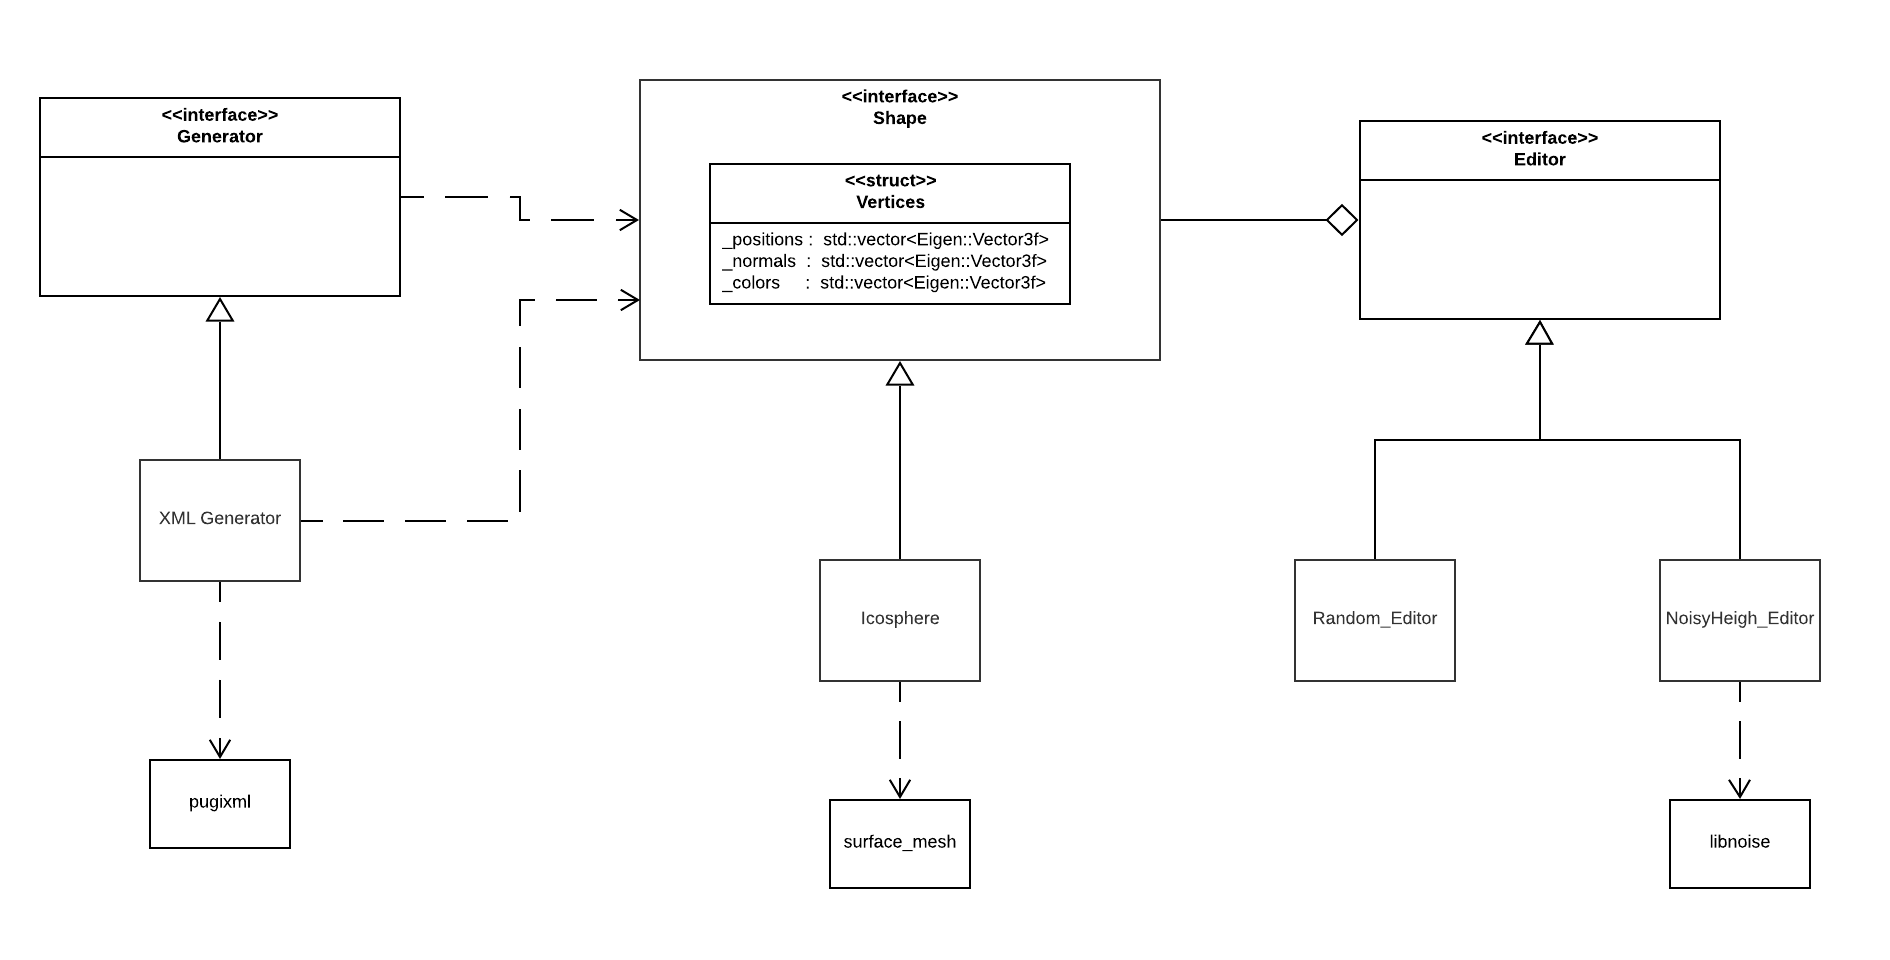
\includegraphics[width=\linewidth]{img/archi/model.png}\end{center}
        \caption{\label{archi_model}Diagramme simplifié du package model}
    \end{figure}

\subsubsection{La représentation d'une planète}

 \begin{figure}[!h]
        \begin{center} 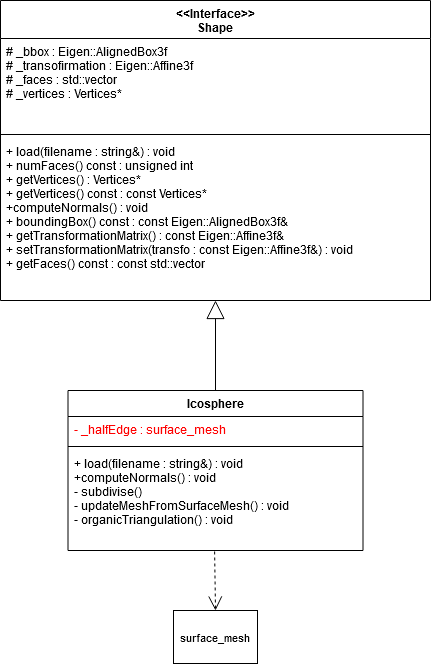
\includegraphics[width=0.5\linewidth]{img/archi/model_shape.png}\end{center}
        \caption{\label{archi_shape}Diagramme simplifié du package model}
    \end{figure}
    
Afin de laissez le choix au développeur d'implémenter de la manière qu'il souhaite une planète, le choix a été fait de faire une interface assez légère. Cette interface est représentée par la figure \ref{archi_shapel}. Elle contient notamment la structure \textbf{Vertices}, utilisé pour stocker l'ensemble des points, leurs normales et les couleurs associés pour permettre la visualisation. Le choix est laissé au développeur d'utiliser la structure de donnée qu'il veut pour gérer la connexité des points. Ainsi, nous limitons alors la dépendance à une bibliothèque en particulier. 
Dans ce projet, c'est une icosphère (icosphere.cpp) qui a été choisie pour représenter une planète sphérique. Pour gérer la connexité des points et des faces, nous avons utilisé la bibliothèque surface\_mesh. En effet, comme nous sommes partis du TD9 de Pierre Benard sur les mondes3D \cite{TD_3D}, une abstraction de la bibliothèque surface\_mesh était proposée. Nous l'avons donc conservé.\\

\subsubsection{Modification d'une planète par un éditeur}

Le choix a été fait de faire une dissociation entre la représentation d'une planète et sa modification. La raison est d'avoir la capacité de créer plusieurs éditeurs de planètes et de pouvoir les appliquer à la même planète de manière cohérente. Cela évite d'autant plus d'avoir un objet beaucoup trop complexe. Une seule méthode doit être implémenter : edit. C'est cette dernière, une fois appelée qui s'occupera de modifier l'ensemble de la planète. Nous mettons à disposition deux éditeurs qui implémentent cette interface : noisyheight\_editor qui produit un bruit de perlin afin de changer le relief et un random\_editor qui lui est complétement aléatoire. Ces deux éditeurs prennent la hauteur des points résultantes afin de leur attribuer une couleur.\\
Une autre conséquence positive de cette séparation est que la forme de départ, l'implémentation de l'interface \textbf{Shape}, peut être ré-implémentée par un autre algorithme que celui que l'on a choisi (\ref{geo_planet}). Ainsi on pourrait remplacé \textbf{Icosphere} par un autre algorithme (voir \ref{algos_gen_sphere}).\\

\subsubsection{Paramètres modifiables par l'utilisateur}

\paragraph{Générateur XML :}

Afin de répondre au besoin \ref{besoin_paramètres} nous avons tout d'abord implémenté un système par ligne de commande. Mais au fur et à mesure de l'avancement, il a été clair que le système était insuffisant à cause du nombre de paramètres et la complexité de ceux-ci.\\
Nous avons donc mis en place une interface \textbf{Generator} dont sa responsabilité est de lire un fichier de configuration, et de créer à la volée la forme de base et appliquer l'éditeur renseigné avec les différents paramètres.
Il retourne ensuite la planète créée qui peut alors être utilisée par la partie visualisation.\\
Cela a permis notamment de faciliter les modifications appliquées par l'utilisateur, pouvant alors librement choisir les paramètres qu'il veut, jusqu'à choisir les paramètres aléatoirement choisi avec la classe \textbf{AleatoryMode} (simple implémentation de bitflags), mais au prix que pour maintenir les nouveaux éditeurs et de nouveaux paramètres, il faut implémenter la lecture de ceux-ci dans les différentes implémentations.\\

L'implémention actuellement de cette interface se fait avec la bibliothèque pugyxml, avec les fichiers de configurations associé (figure \ref{archi_generator}).
    \begin{figure}[!h]
        \begin{center} 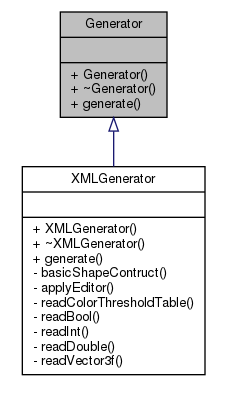
\includegraphics[width=0.3\linewidth]{img/archi/archi_generator.png}\end{center}
        \caption{\label{archi_generator}Diagramme de classe simplifié de Generator et ses implémentations (doxygen).}
    \end{figure}
    
On a gardé cependant la possibilité dans le main de changer le comportement par défaut si il n'y a pas de fichier de configuration, ce qui permet de garder l'extensibilité mais nécessite une recompilation du programme à chaque modification.

\paragraph{Couleurs paramétrables :}

Lié au besoin de l'implémentation précédente, il a fallu créé un système qui puisse déterminer sur une échelle de hauteur les couleurs à utiliser dans les éditeurs (figure \ref{archi_treshold}).

Plus généralement, on pourrait étendre ce principe pour une échelle de valeurs d'un paramètre, où il faut découper son domaine et associer à chacun une donnée arbitraire (ou non). C'est ce principe qu'illustre la classe \textbf{TresholdTable}, qu'on utilise pour les tables de couleurs selon une hauteur par convention dans [-1,1], mais comme c'est une classe template elle serai extensible à d'autres problèmes, souvent liés à la décidabilité des biômes suivant un paramètre (voire plusieurs si on fait des tables à plusieurs dimensions imbriquées).

\begin{figure}[!h]
        \begin{center} 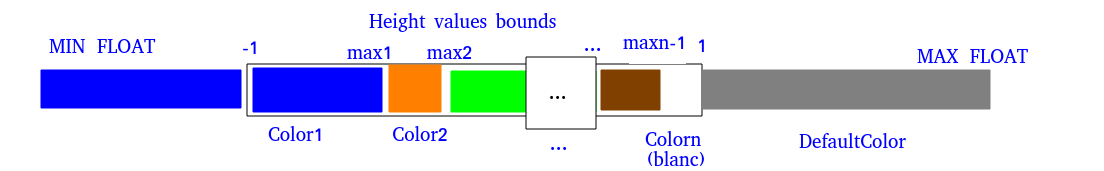
\includegraphics[width=\linewidth]{img/archi/example_treshold.png}\end{center}
        \caption{\label{archi_treshold}Principe illustré avec des couleurs de la classe TresholdTable.}
\end{figure}

\newpage
\subsubsection{Aléatoire et bruit}

Afin d'avoir une sorte de boite à outil pour tout ce qui concerne l'aléatoire et les bruits, nous avons créé le namespace \textbf{NoiseRandom}. Il permet de centralisé les fonctions global facilitant la manipulation de l'aléatoire, mais aussi grâce à la classe \textbf{HeightNoise} au sien de ce namespace de fournir une abstraction de la bibliothèque Libnoise et de séparer cette dépendance. Au cas où on utiliserait une autre bibliothèque, on pourrait ainsi en changeant l'implémentation de HeightNoise impacter de façon minimal le reste du code si on change pas les signatures de fonction.

\subsection{Visualisation}

% Mettre une image de l'architecture ici

La visualisation, comme son nom l'indique, regroupe l'ensemble des classes permettant l'affichage et l'interaction avec l'utilisateur. L'ensemble de ses classes est présent dans le %package view. % Pas de package en C++
L'affichage devait se faire sur un système d'exploitation Linux, il a donc été choisi de le faire via OpenGL. Pour éviter néanmoins toute dépendance avec, et donc permettre toute extension (via Windows avec DirectX par exemple), on a utilisé le pattern bridge via l'interface Rendering. Cette dernière est implémentée par Rendering\_OpenGL. Toute fonction de visualisation de la planète passe donc par cette interface. Elle est principalement utilisée dans la classe \textbf{Viewer}, qui s'occupe à la fois de générer une visualisation mais aussi des interactions avec l'utilisateur (déplacement de la caméra et zoom principalement). Ces interactions sont gérées ici par la bibliothèque GLFW.
La capacité de déplacement de l'affichage est faite par l'intermédiaire de la classe caméra qui hérite de trackball, cette dernière contenant l'ensemble des méthodes nécessaires au zoom et à la rotation, ainsi qu'aux matrices de projections.

\subsection{Récapitulatif des dépendances}

\paragraph{Mozilla Public License 2 : }
\begin{itemize}
\item Eigen :  
     Facilite les calculs matriciels pour la géométrie. 
 \item glbinding :  
     Permet le lien entre les données en mémoire et Opengl.
\item glfw : 
     API utilisé pour la gestion de fenêtre et les intéractions clavier.
\end{itemize}

\paragraph{GNU Library General Public License, Version 2 : }
\begin{itemize}
\item surface\_mesh :
    Facilite la gestion de connectivité et connexité des vertices pour la subdivision. Copyright (C) 2013 by Graphics \& Geometry Group, Bielefeld University
\item Libnoise :
    Utilisé pour créer les reliefs à partir de bruits cohérents.
\end{itemize}

\paragraph{MIT License :}
\begin{itemize}
\item pugyxml:
    Permet la prise en charge de fichiers de configurations xml.
\end{itemize}

\paragraph{Copyright 2008, Google Inc. :}
\begin{itemize}
\item Googletest :
    Permet de facilité la mise en place de tests unitaires automatisés. 
\end{itemize}

\newpage 
\section{Analyse du fonctionnement}

La figure \ref{seqmodel} représente le diagramme de séquence de la partie modèle. 
On peut voir ainsi tout d'abord la lecture du fichier de configuration par l'objet XMLGenerator qui va ensuite le long de la lecture renseignée tout les paramètres d'abord pour créer la géométrie de base, ici une icosphère, et ensuite la modifier avec un éditeur, par exemple NoisyHeight\_Editor. Cas spécial, si le paramètre n'existe pas dans le fichier pour l'éditeur on choisira le paramètre aléatoirement grâce au renseignement par un système de "flags" dans le constructeur, Icosphere n'ayant que des valeurs par défaut dans ce cas là, il n'en a pas besoin. A la fin on donnera la planète obtenu à la partie visualisation avec au passage l'affichage des paramètres.\\

\begin{figure}[!h]
\centering
 \makebox[\textwidth][c]{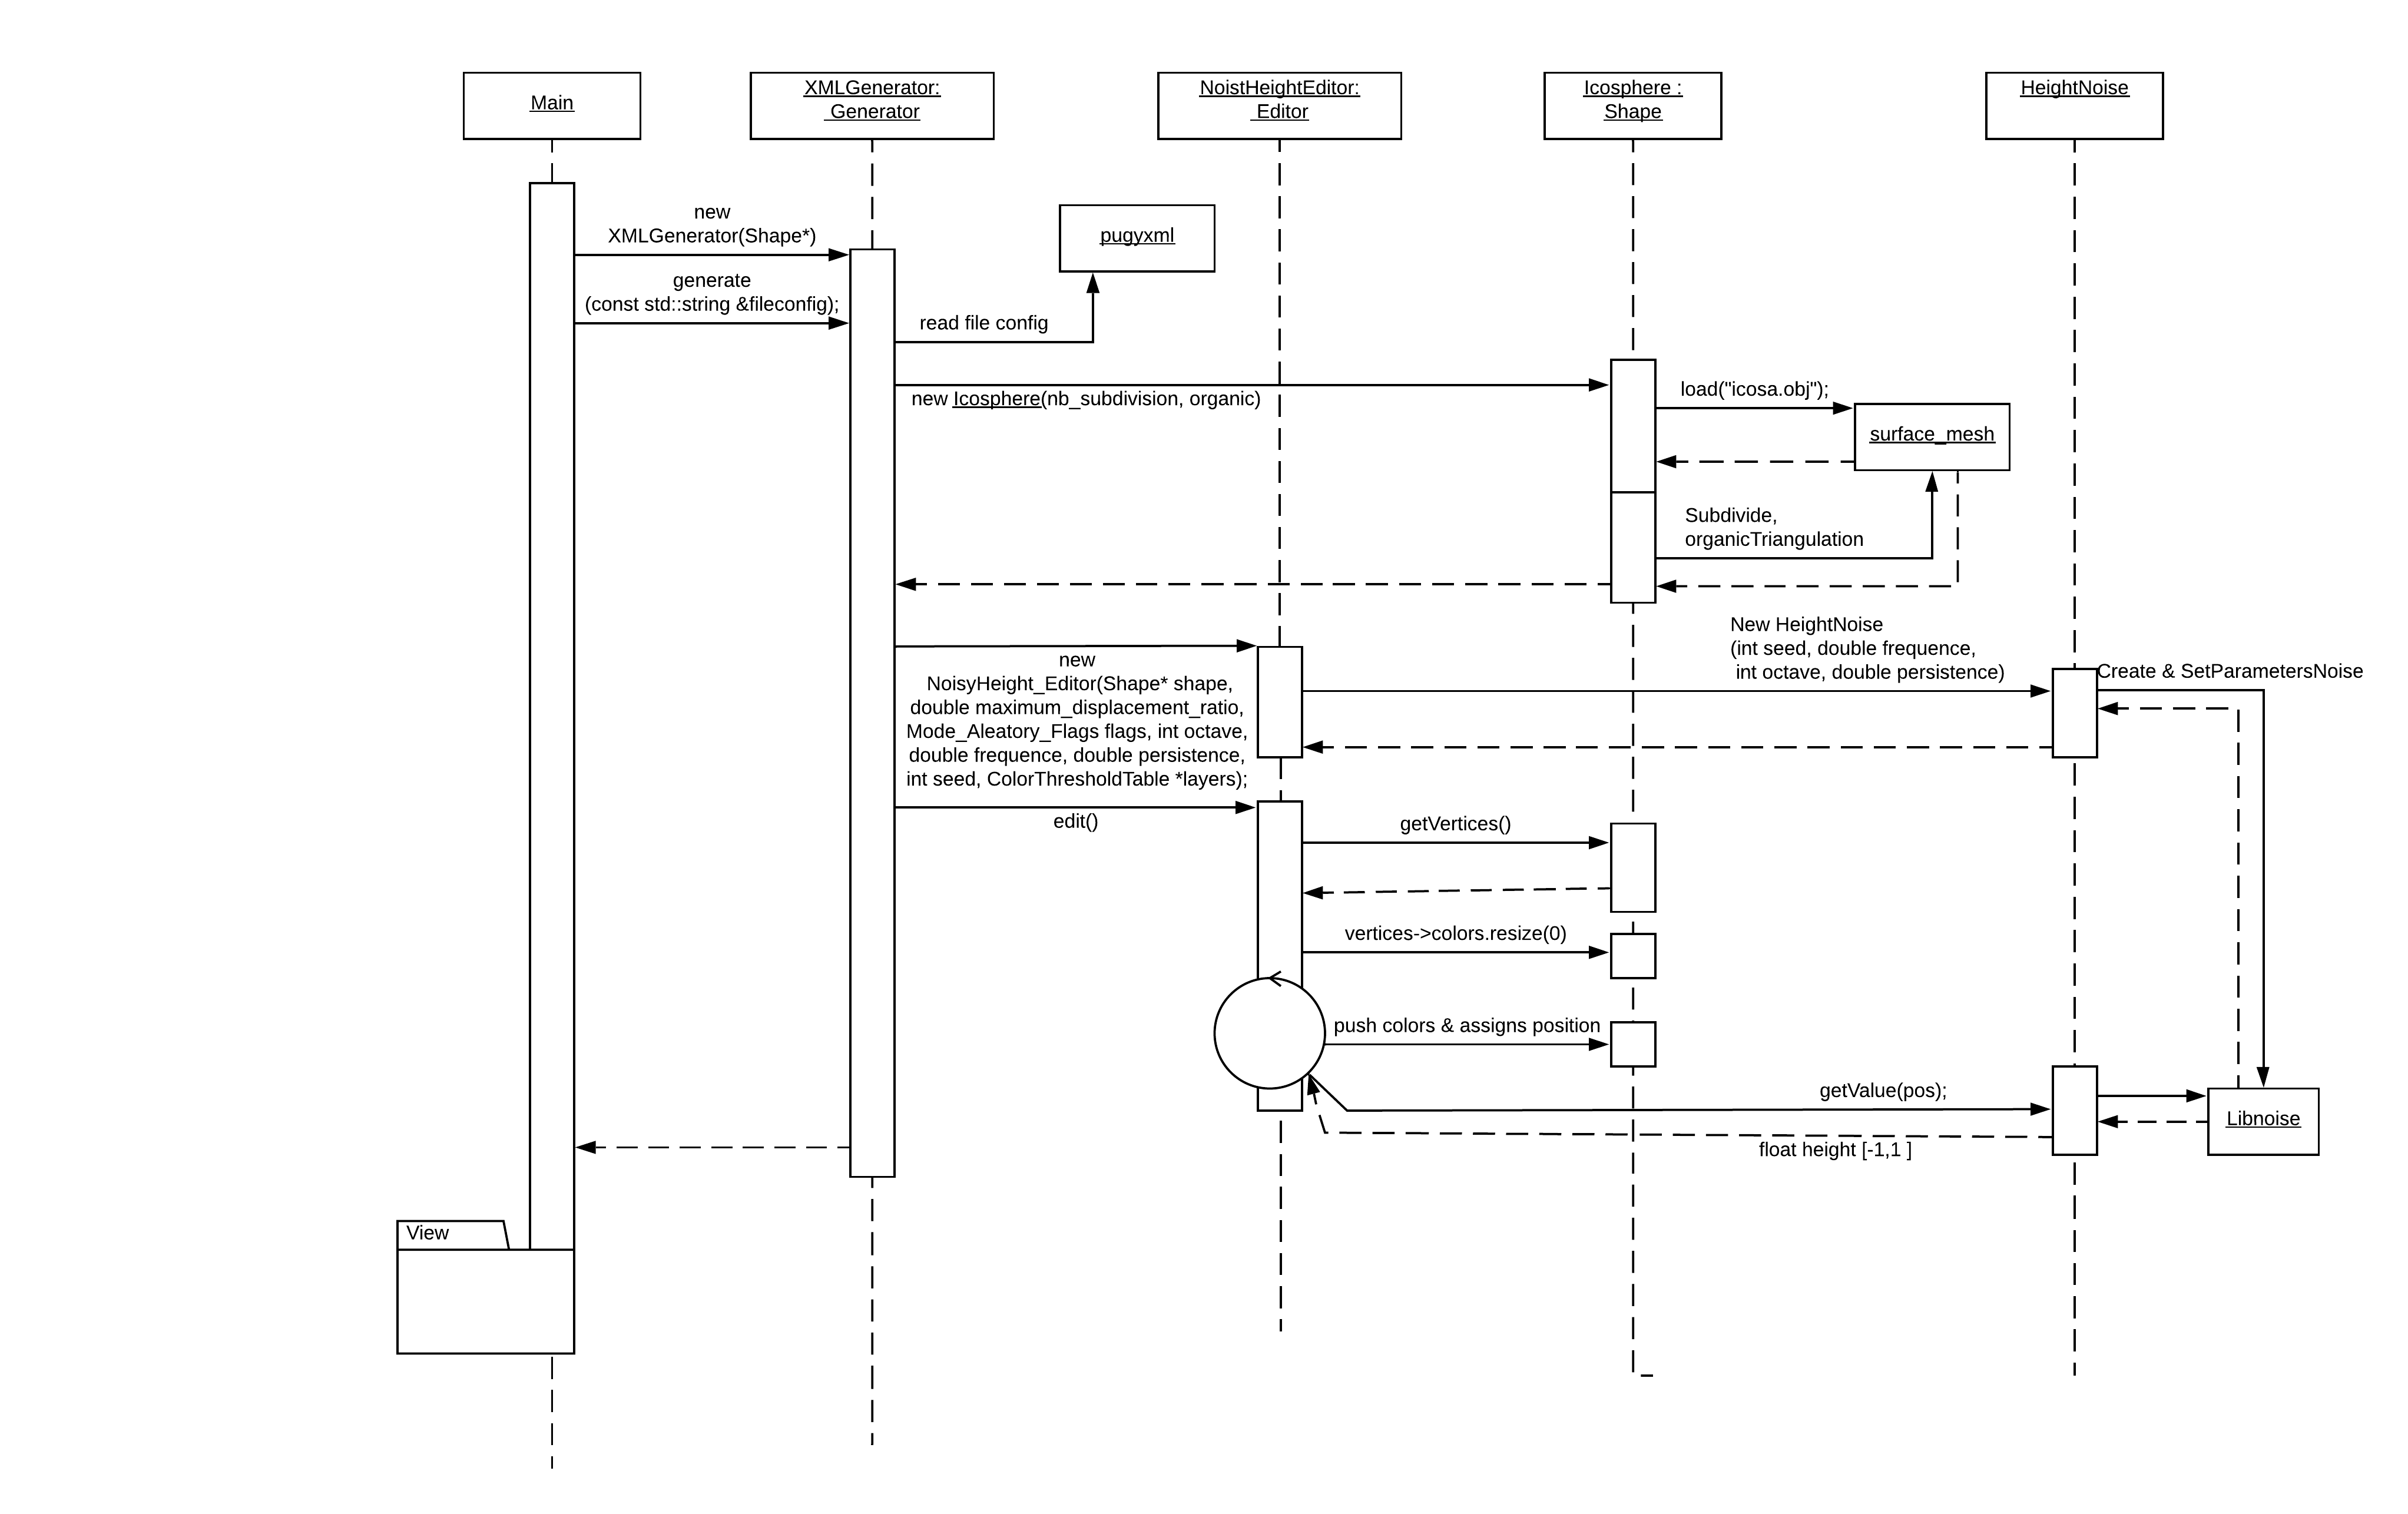
\includegraphics[width = 1.2\textwidth]{img/seqmodel.png}}
\caption{Diagramme de séquence de la partie model.}
\label{seqmodel}
\end{figure}

Ensuite on crée une fenêtre OpenGL grâce à GLFW, et on envoie les informations géométriques et graphiques de la planète au GPU pour manipuler la représentation via le vertice shader et le fragment shader (renseigné dans src/data/shaders/) afin de permettre l'affichage dans cette même fenêtre. Les shaders reçoivent les informations pour chaque sommet (position, normale, couleur) et les interprètent afin de savoir quelle couleur afficher, en utilisant la théorie d'éclairage de Blinn-phong. L'affichage est ensuite constamment actualisée, afin de permettre l'interaction avec l'utilisateur.
Pour les mers et les océans nous utilisation un mode conditionnel particulier du shader afin de ne pas copier une sphère de base pour la surface transparente. Autrement dit, on fait l'affichage en 2 passes avec d'abord la planète modifié sans les océans, et ensuite on refait une passe via ce mode pour aplatir dans le GPU le relief, et appliquer une couleur prédéfini dans le shader. Nous pouvons ainsi gagner en mémoire et en temps si on devait le faire sur CPU.

La figure \ref{seqvisu} montre le diagramme de séquence de la partie visualisation.

\begin{figure}[!h]
    \begin{center}
        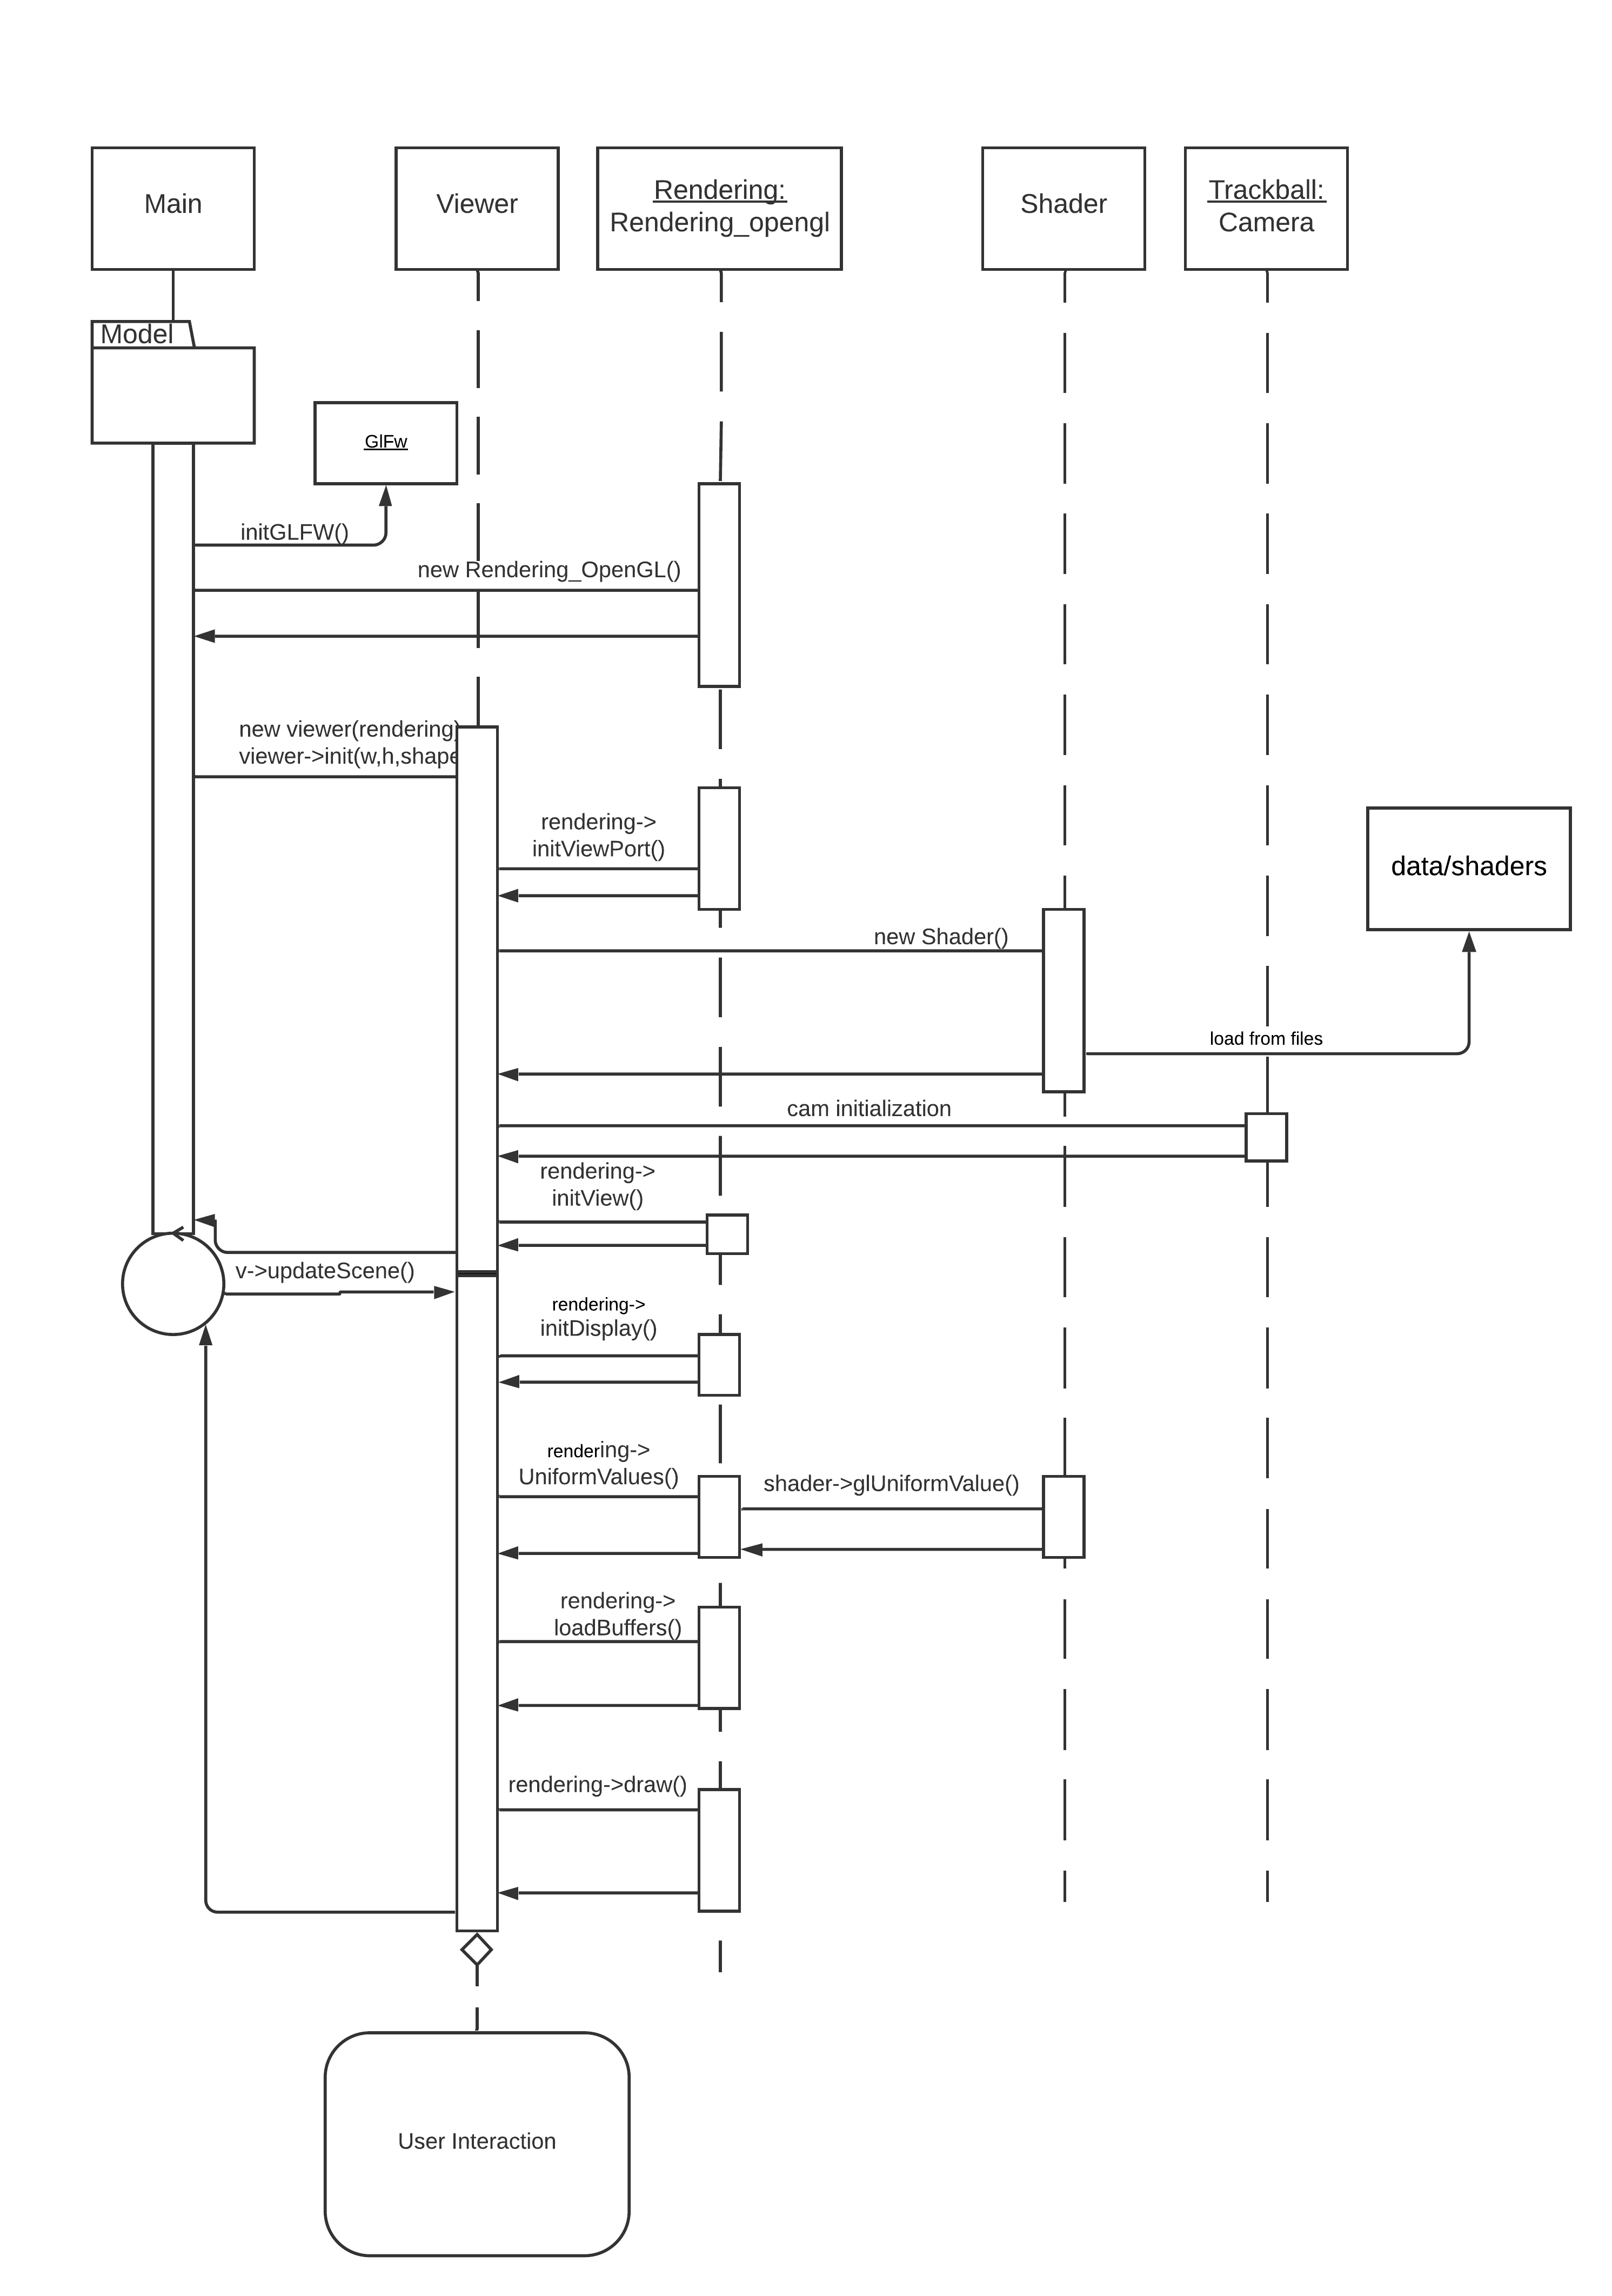
\includegraphics[width=0.7\linewidth]{img/visu_seq.png} 
        \caption{Diagramme de séquence de la partie visualisation.}
        \label{seqvisu}
    \end{center}
\end{figure}

\newpage
A tout moment, l'utilisateur peut faire tourner la planète à l'aide de la souris (en cliquant et glissant dans la fenêtre), et effectuer un zoom/dézoom sur la planète. Il peut également appuyer sur S pour sauvegarder et W pour afficher le maillage en mode fil de fer. Ces interactions sont détaillés dans la figure \ref{seqinter} 

\begin{figure}[!h]
    \begin{center}
        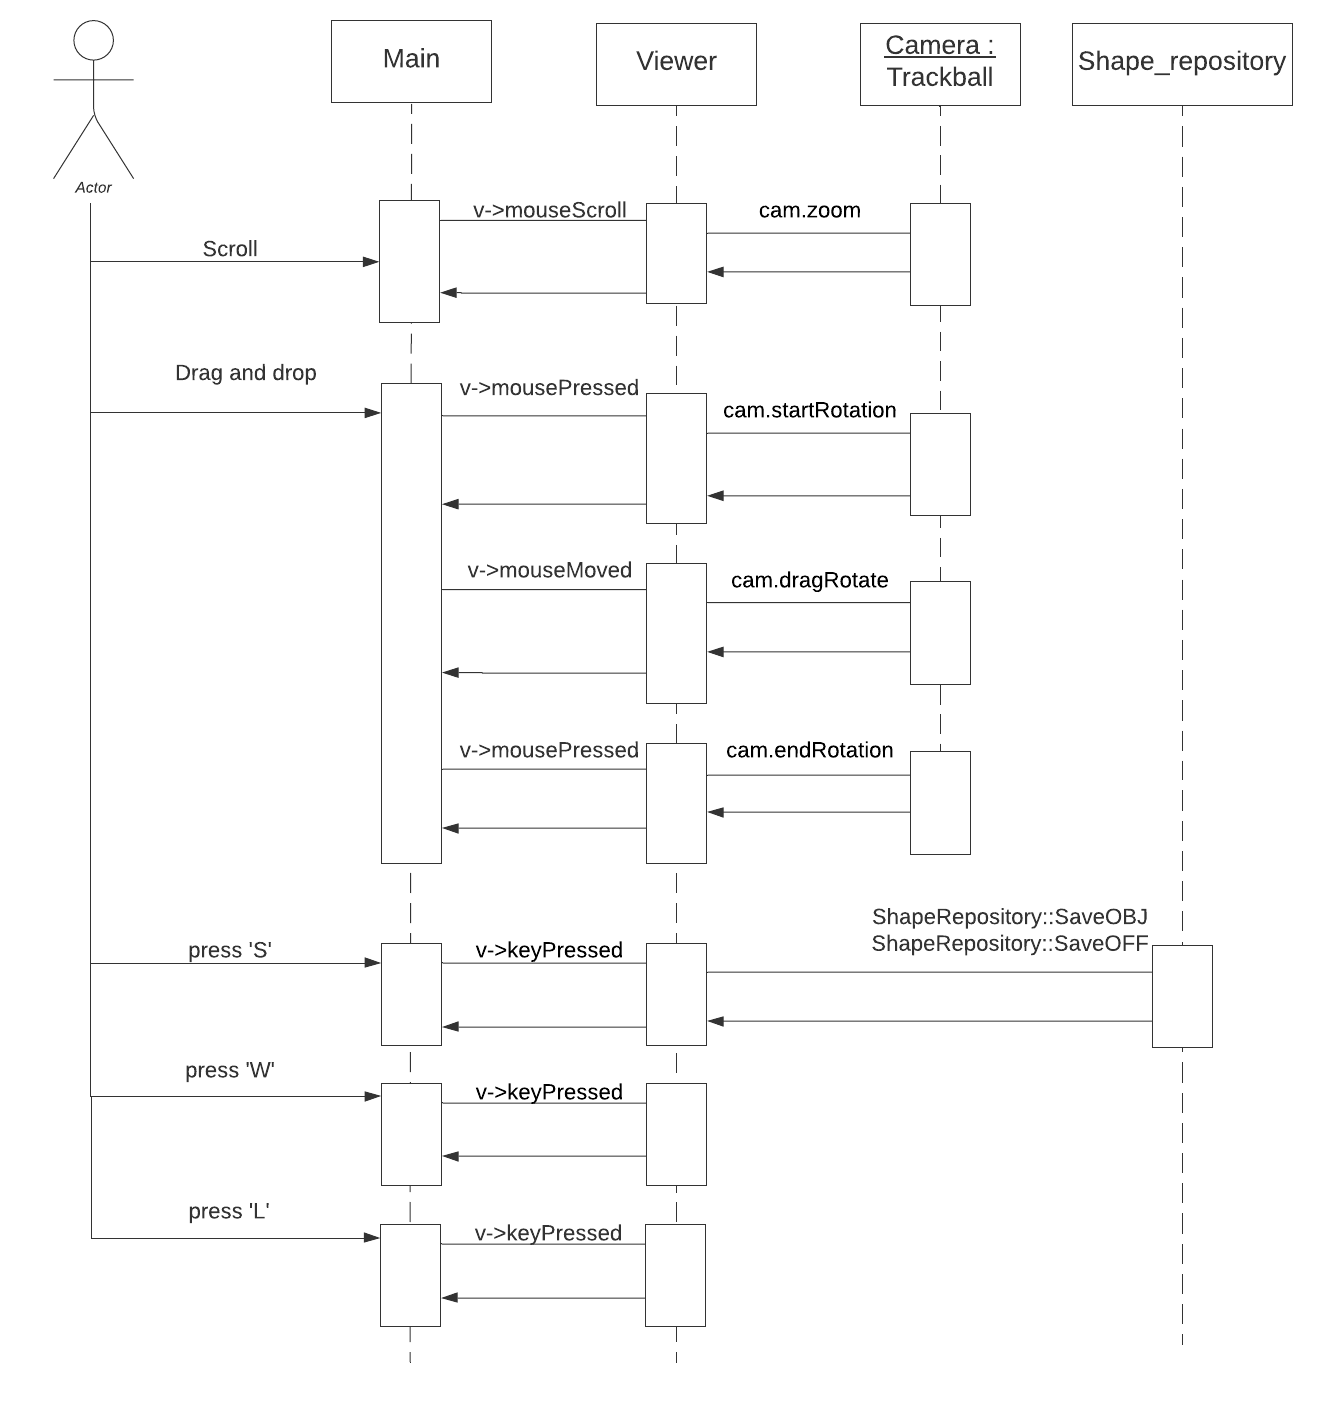
\includegraphics[width=0.7\linewidth]{img/interaction_seq.png} 
        \caption{Diagramme de séquence de la partie interaction.}
        \label{seqinter}
    \end{center}
\end{figure}

\newpage
Après exécution de notre logiciel avec le fichier de configuration "simple.xml", on obtiens une planète comme la figure \ref{notre_planete}. On peut lire ensuite dans le terminal les différents paramètres qui ont été utilisé afin de créer un fichier de configuration avec les mêmes paramètres pour pouvoir la recréer et faire de légers ajustements.\\

\begin{figure}[!h]
    \begin{center}
        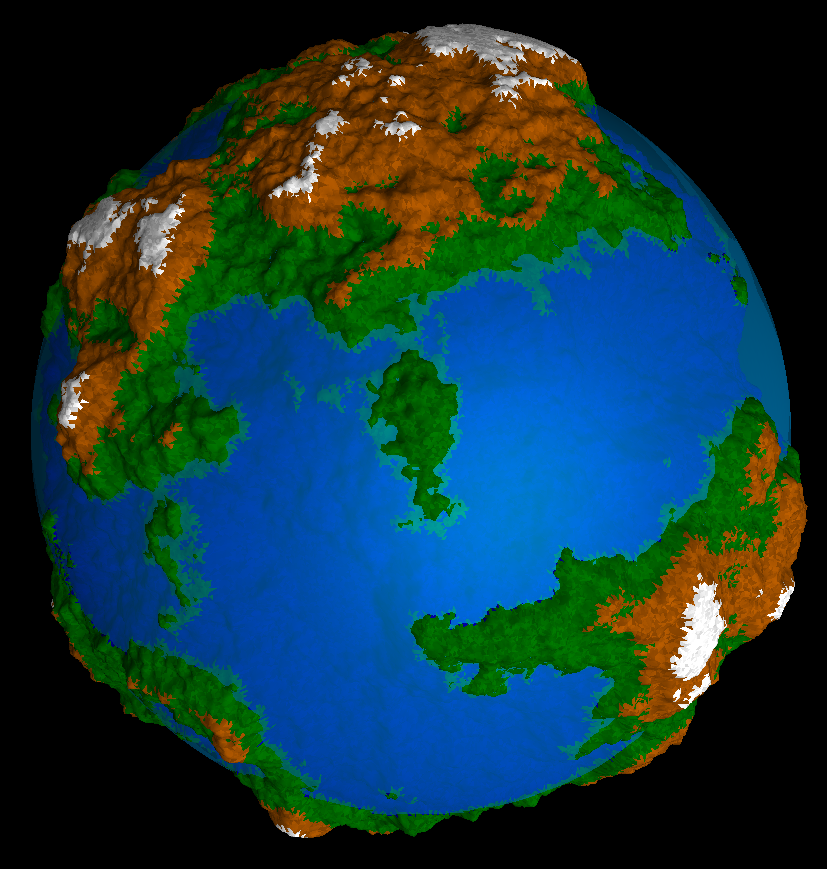
\includegraphics[width=0.6\linewidth]{img/notre_planete.png} 
        \caption{Une planète générée à partir de "simple.xml"}
        \label{notre_planete}
    \end{center}
\end{figure}


\newpage 
\section{Tests}

 A METTRE EN VALEUR
 (1) specification et buts du test ; (2) cas de test (donnees utilisees) ; (3) scenarios de tests ; (4) analyse du test
Utilisation de google test

\subsection{Tests esthétiques}

%RDV Client A détailler
RDV Client A détailler et scénarios qualitatifs

\subsection{Tests sur les éditeurs}

Le test sur les éditeurs concerne principalement le seul éditeur paramétrable et où l'aléatoire n'entre pas trop en compte. En effet, il est difficile de tester que fonctionne correctement un éditeur où tout est aléatoire (cas du random\_editor). Dans le cas du noisyheight\_editor, il est possible de vérifier qu'il fonctionne correctement. En effet, à paramètres équivalent, la génération doit être identique au niveau de la position des points et des normals. (Pas le cas des couleurs qui peuvent légèrement varier au vu de la palette disponible). Pour se faire, nous procédons à deux générations de planète avec les mêmes paramètres, puis nous comparons la valeurs de chaque point dans le tableau de position. Nous faisons la même chose pour les normales. Si les deux sont parfaitement identique, la génération est alors correct.

\subsection{Tests sur les performances}

On cherche ici à évaluer les performances de calcul en fonction du nombre de subdivision et de l'application de notre éditeur. Pour cela on répète la création pour une valeur de subdivision afin d'avoir une moyenne par valeur de subdivision, et on augmente la subdivision. On peut alors savoir jusqu'où il est possible d'aller dans le nombre de subdivision si on ne donne pas de bornes supérieur. On compare aussi le temps de calcul avec et sans editeur, en fonction du nombre de subdivision et nous obtenons alors le graphique visibile à la figure \ref{graphperf}

\begin{figure}[!h]
    \begin{center}
        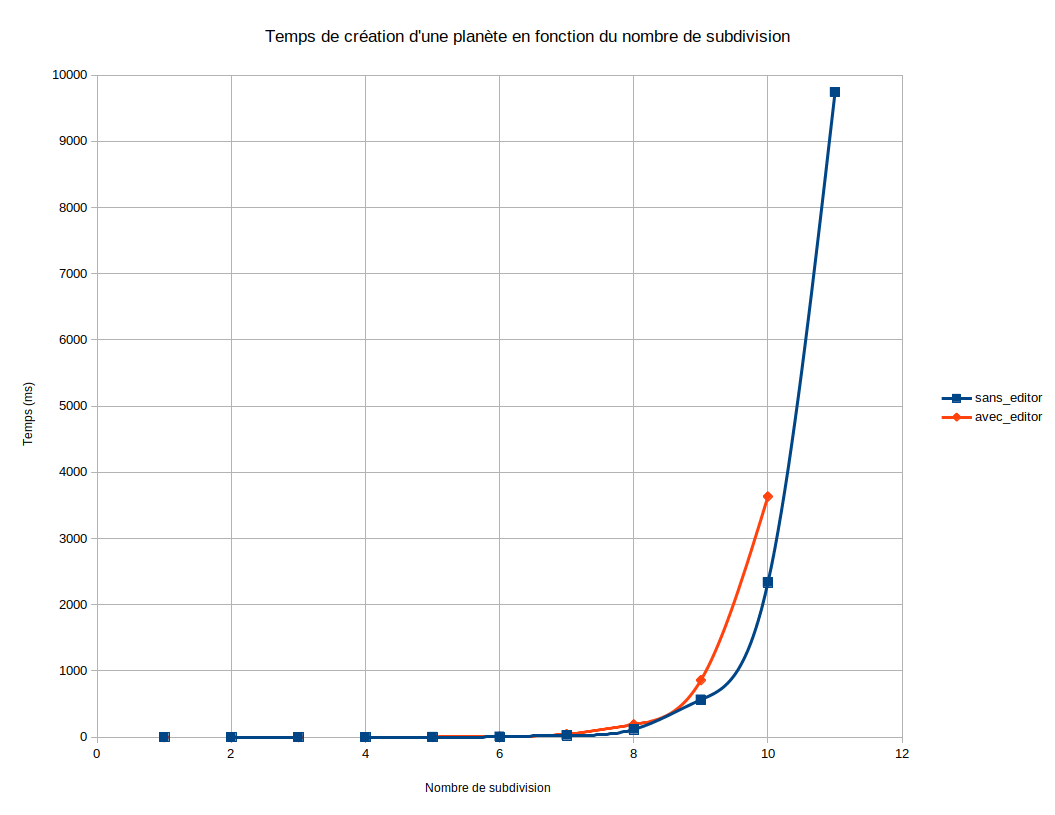
\includegraphics[scale=0.4]{img/perf.png}
        \caption{Graphique représentant le temps de génération en fonction du nombre de subdivision et l'application ou non d'un éditeur\protect\footnotemark}
        \label{graphperf}
    \end{center}
\end{figure}

On remarque alors que passé la subdivision de taille 10, le temps commence à augmenter de manière exponentiel. Même si 10 secondes restent tout à fait raisonnable, si on va plus loin le test nous a permis de mettre en évidence le manque de mémoire afin de réaliser la génération qui se solde par une exception de "bad alloc".

% Pistes d'améliorations et complexité analyse
% Nombre de faces = combien de subdivisions ?

\subsection{Test sur le temps de génération}

Le but de ce test est de déterminer le nombre de subdivision possible dans un certain temps donné. Ainsi, on cherche à obtenir avec ce test quel est le nombre de subdivision idéal dans un temps arbitraire( que l'on peut voir comme une contrainte du client). On part donc d'une subdivision à 0, et on augmente tant que le temps ne dépasse pas celui que l'on souhaite avoir. Dans le cas de notre test, on prend en compte le temps de modification de la planète à lui appliquant le NoiyHeight\_Editor.

\subsection{Test sur la sauvegarde}

Pour s'assurer que la sauvegarde fonctionne correctement, il faut s'assurer que les données sauvegarder soient identiques à la planète qui a été générée. Pour se faire, nous mettons en place un test scénario. Nous sauvegarder dans les données au sein d'un fichier .obj que nous lançons sur un logiciel de visionnage (type blender). Si le fichier n'est pas correct, il est facile de l'observer car la planète générée ne sera pas du tout la même. Il est tout à fait possible de sauvegarder la planète 2 fois et vérifier que les données soient les mêmes, mais ce genre de test ne garantie pas que les données sauvegardées soient les bonnes. La seul référence possible est une référence visuel. Nous pouvons tout à fait lancer le fichier depuis notre exécutable pour comparer que les deux planètes sont identiques (il n'est donc pas forcément nécessaire d'utiliser un logiciels tiers pour comparer).

\subsection{Tests de non régression}

\paragraph{Coordonnées : } On a vérifié le bon passage des coordonnées cartésiennes à sphériques, et vice versa, tantôt avec des valeurs d'oracle, tantôt avec des valeurs aléatoires où on doit pouvoir revenir à la cordonnées de départ.
On a aussi vérifie certains points particulier comme 

\paragraph{Random : } On a vérifié que pour les fonctions de hasard suivent bien le comportement indiqué, autant sur les domaines que sur les lois qu'elles doivent suivre selon la loi des grands nombres.

\paragraph{Treshold : } On a vérifié la bonne construction et l'ordre des couches dans la table ainsi que la non-modification des données durant le processus. 
On a testé aussi si sur une valeur comprise dans l'intervalle du minimum et du maximum des bornes de la tables la fonction getColorDataByValue renvoie bien la bonne donnée de la couche auquel cette valeur appartient.
Comme le nombre de couches et les données sont non importantes pour ces tests, c'est décidé aléatoirement.

\subsection{Tests mémoires}

Nous nous sommes assuré des fuites mémoires avec l'outil Valgrind, à la fois sur les tests et sur le programme principal.
Conclusion nous n'avons pas de problèmes majeurs de mémoire, bien que des avertissements d'utilisation de variables non-initialisé soit présent du à la bibliothèque, et des erreurs ressorte de GLFW de possible oubli de libération avec GLFW dont on a pas le contrôle.

\section{Conclusion}
% description de ce qu’il y aurait encore `a faire,extensions (et comment les réaliser).
% et besoins non satisfaits

\section{Annexes}

\begin{figure}[!h]
    \begin{center}
        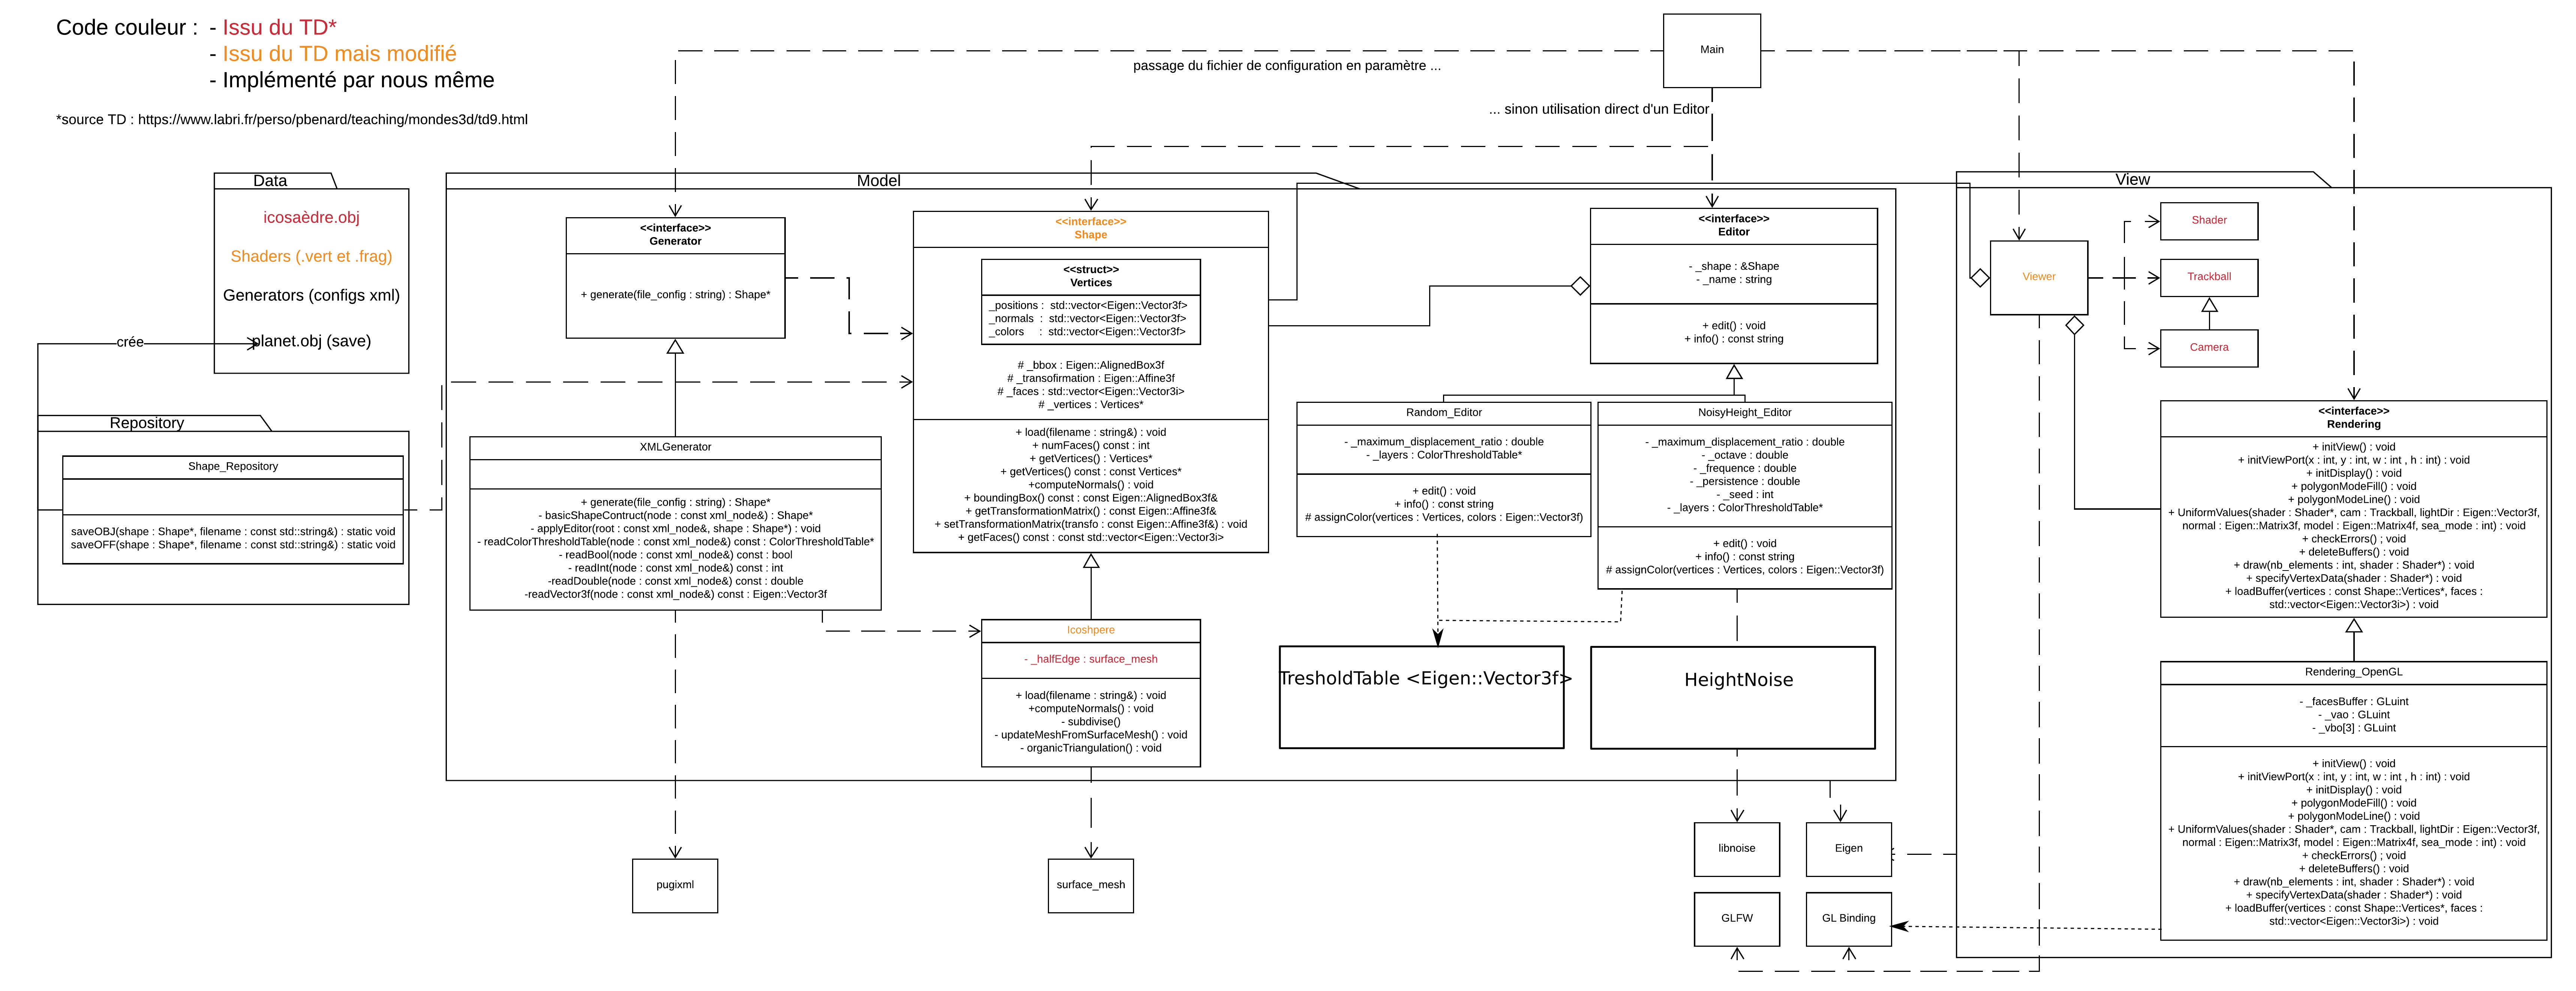
\includegraphics[width=1.5\linewidth, angle=90]{img/archi/Architecture_complete.png} 
        \caption{Architecture complète}
        \label{archiComplete}
    \end{center}
\end{figure}

%----------------------------------------------------------------------------------------

\bibliographystyle{plain}
\bibliography{bibliographie}

\end{document}
